% !TeX root = doc_pi1.tex
\documentclass[12pt,openright,oneside,a4paper,english,french,spanish,brazil]{abntex2}
\usepackage{cmap}
\usepackage{longtable}
\usepackage{lmodern}	
\usepackage[T1]{fontenc}	
\usepackage[utf8]{inputenc}		
\usepackage{lastpage}		
\usepackage{indentfirst}
\usepackage{color}	
\usepackage{graphicx}	
\usepackage{units}
\usepackage[brazilian,hyperpageref]{backref}
\usepackage[alf]{abntex2cite}
\usepackage{bold-extra}
\usepackage{eso-pic}
\usepackage{pdflscape}
\usepackage{hyperref}
\usepackage{makecell}
\usepackage{tabularx}  % Para tabelas com largura ajustável
\usepackage{booktabs}  % Para linhas de tabela mais profissionais 
\renewcommand{\backrefpagesname}{Citado na(s) página(s):~}
\renewcommand{\backref}{}
\renewcommand*{\backrefalt}[4]{
	\ifcase #1 %
		Nenhuma citação no texto.%
	\or
		Citado na página #2.%
	\else
		Citado #1 vezes nas páginas #2.%
	\fi}%
% ---


\usepackage{fixos/customizacoes}
\usepackage{cancel}
\usepackage{amsmath}
\usepackage{amssymb}
\usepackage{float}
\usepackage{url}
\usepackage[hyphens]{url} % para permitir quebra automática em hífens
\usepackage{hyperref}     % se quiser links clicáveis



% Dados pessoais
\autor{Alberto Côrtes, Arthur Ribeiro, Caio Soares, Carlos Eduardo Rodrigues, Davi Rodrigues, David William, Ingrid Alves, João Guilherme Capozzi, João Guilherme Veras, Leticia Maria, Liz Stella Cunha, Lucas Machado, Marcos Filho, Mariana Pereira, Mariana Ribeiro, Rayene Ferreira, Patricia Helena Macedo e Víctor Moreira}
\curso{}

% Dados do trabalho
\titulo{Projeto de PI1}
\data{2025}
\palavraChaveUm{Projeto Integrador de Engenharia 1}
\palavraChaveDois{Faculdade de Ciências e Tecnologias em Engenharia}
\palavraChaveTres{Foguetes d'água}
\palavraChaveQuatro{Controle de trajetória}
\palavraChaveCinco{Sistema embarcado}
% Dados da orientacao
\orientador{Prof. Lui Txai Calvoso Habl}
\coorientador{Prof. Juliana Petrocchi, Prof. Diogo Caetano, Prof. Ricardo Ajax e Prof. Rafael Rodrigues}

% % Dados para a ficha catalográfica
% \cdu{02:141:005.6}

% % Dados da aprovação do trabalho
% \dataDaAprovacao{01 de junho de 2013 -- Data da aprovação do trabalho}
% \membroConvidadoUm{Titulação e Nome do Professor Convidado 01}
% \membroConvidadoDois{Titulação e Nome do Professor Convidado 02}

\local{Brasília, DF}
\instituicao{%
  Universidade de Brasília -- UnB
  \par
  Faculdade UnB Gama -- FGA
}
\tipotrabalho{Projeto Integrador de Engenharia 1}
\preambulo{ Trabalho submetido à disciplina de Projeto Integrador de Engenharia 1 %Monografia submetida ao curso de graduação em \imprimircurso\ 
da Universidade de Brasília.} %, como requisito parcial para obtenção do Título de Bacharel em \imprimircurso.}

\definecolor{blue}{RGB}{41,5,195}
\makeatletter
\hypersetup{
     	%pagebackref=true,
		pdftitle={\@title}, 
		pdfauthor={\@author},
    	pdfsubject={\imprimirpreambulo},
	    pdfcreator={LaTeX with abnTeX2},
		pdfkeywords={abnt}{latex}{abntex}{abntex2}{trabalho acadêmico}, 
		colorlinks=true,       		% false: boxed links; true: colored links
    	linkcolor=blue,          	% color of internal links
    	citecolor=blue,        		% color of links to bibliography
    	filecolor=magenta,      		% color of file links
		urlcolor=blue,
		bookmarksdepth=4
}
\makeatother
\setlength{\parindent}{1.3cm}
\setlength{\parskip}{0.2cm}  
\makeindex


\begin{document}

\frenchspacing 
\imprimircapa
\imprimirfolhaderosto* {}

\begin{fichacatalografica}
	\vspace*{\fill}					% Posição vertical
	\hrule							% Linha horizontal
	\begin{center}					% Minipage Centralizado
	\begin{minipage}[c]{12.5cm}		% Largura
	
	\imprimirautor
	
	\hspace{0.5cm} \imprimirtitulo  / \imprimirautor. --
	\imprimirlocal, \imprimirdata-
	
	\hspace{0.5cm} \pageref{LastPage} p. : il. (algumas color.) ; 30 cm.\\
	
	\hspace{0.5cm} \imprimirorientadorRotulo~\imprimirorientador\\
	
	\hspace{0.5cm}
	\parbox[t]{\textwidth}{\imprimirtipotrabalho~--~\imprimirinstituicao,
	\imprimirdata.}\\
	
	\hspace{0.5cm}
		1. \imprimirpalavrachaveum.
		2. \imprimirpalavrachavedois.
		I. \imprimirorientador.
		II. Universidade de Brasília.
		III. Faculdade UnB Gama.
		IV. \imprimirtitulo\\ 			
	
	\hspace{8.75cm} CDU \\ %\nomecdu\\
	
	\end{minipage}
	\end{center}
	\hrule
        \pagebreak
\end{fichacatalografica}


% \begin{errata}
Elemento opcional da \citeonline[4.2.1.2]{NBR14724:2011}. \textbf{Caso não 
deseje uma errata, deixar todo este arquivo em branco}. Exemplo:

\vspace{\onelineskip}

FERRIGNO, C. R. A. \textbf{Tratamento de neoplasias ósseas apendiculares com
reimplantação de enxerto ósseo autólogo autoclavado associado ao plasma
rico em plaquetas}: estudo crítico na cirurgia de preservação de membro em
cães. 2011. 128 f. Tese (Livre-Docência) - Faculdade de Medicina Veterinária e
Zootecnia, Universidade de São Paulo, São Paulo, 2011.

\begin{table}[htb]
\center
\footnotesize
\begin{tabular}{|p{1.4cm}|p{1cm}|p{3cm}|p{3cm}|}
  \hline
   \textbf{Folha} & \textbf{Linha}  & \textbf{Onde se lê}  & \textbf{Leia-se}  \\
    \hline
    1 & 10 & auto-conclavo & autoconclavo\\
   \hline
\end{tabular}
\end{table}

\end{errata}
 
% \begin{folhadeaprovacao}

  \begin{center}
    {\ABNTEXchapterfont\large\imprimirautor}

    \vspace*{\fill}\vspace*{\fill}
    {\ABNTEXchapterfont\bfseries\Large\imprimirtitulo}
    \vspace*{\fill}
    
    \hspace{.45\textwidth}
    \begin{minipage}{.5\textwidth}
        \imprimirpreambulo
    \end{minipage}%
    \vspace*{\fill}
   \end{center}
    
   Trabalho aprovado. \imprimirlocal, \imprimirdatadaaprovacao:

   \assinatura{\textbf{\imprimirorientador} \\ Orientador} 
   \assinatura{\textbf{\imprimirmembroconvidadoum} \\ Convidado 1}
   \assinatura{\textbf{\imprimirmembroconvidadodois} \\ Convidado 2}
      
   \begin{center}
    \vspace*{0.5cm}
    {\large\imprimirlocal}
    \par
    {\large\imprimirdata}
    \vspace*{1cm}
  \end{center}
  
\end{folhadeaprovacao}

% \begin{dedicatoria}
   \vspace*{\fill}
   \centering
   \noindent
	\textbf{A dedicatória é opcional. Caso não deseje uma, deixar todo este
	arquivo em branco}.

   \textit{Este trabalho é dedicado às crianças adultas que,\\
   quando pequenas, sonharam em se tornar cientistas.} \vspace*{\fill}
\end{dedicatoria}

% \begin{agradecimentos}
A inclusão desta seção de agradecimentos é opcional, portanto, sua inclusão 
fica a critério do(s) autor(es), que caso deseje(em) fazê-lo deverá(ão) 
utilizar este espaço, seguindo a formatação de \textit{espaço simples e 
fonte padrão do texto (sem negritos, aspas ou itálico}.

\textbf{Caso não deseje utilizar os agradecimentos, deixar toda este arquivo
em branco}.
\end{agradecimentos}

% \begin{epigrafe}
    \vspace*{\fill}
	\begin{flushright}
		\textbf{A epígrafe é opcional. Caso não deseje uma, deixe todo
		este arquivo em branco}.

		\textit{``Não vos amoldeis às estruturas deste mundo, \\
		mas transformai-vos pela renovação da mente, \\
		a fim de distinguir qual é a vontade de Deus: \\
		o que é bom, o que Lhe é agradável, o que é perfeito.\\
		(Bíblia Sagrada, Romanos 12, 2)}
	\end{flushright}
\end{epigrafe}


\begin{resumo}
% \textcolor{red}{O resumo é um item obrigatório. Essa parte do relatório será uma visão rápida e clara do projeto desenvolvido. O leitor terá informações como: descrição breve do projeto, principais requisitos, tecnologias necessárias e outras informações relevantes para apresentação. O resumo terá no máximo meia (1/2) página.}

% \textcolor{red}{Ao longo deste texto, as descrições em \textbf{cor vermelha} são meras instruções, não devendo aparecer na versão final do texto. \textbf{Utilize o comentário \% ao invés de apagar estas descrições, para não perder as orientações apresentadas.}}

\tab{1cm}O presente projeto visa o desenvolvimento de um foguete d'água reutilizável com sistema de controle de trajetória, projetado para lançamentos em distâncias fixas de 10m, 20m e 30m com margem de precisão de 0,5m. A proposta inclui a integração de um sistema embarcado responsável pela realização de medições em tempo real por meio de hardware, com posterior apresentação e análise dos dados via software. Entre os parâmetros monitorados estão a altura, a velocidade, o ângulo de lançamento e o volume de água, é notório que a coleta precisa desses dados é de suma importância para garantir estimativas coerentes com os requisitos de distância definidos. Este projeto tem aplicação educacional e experimental, promovendo aprendizado em áreas práticas como física, aerodinâmica e sistemas embarcados, com foco na reusabilidade, confiabilidade e precisão.

\vspace{\onelineskip}
\noindent
\textbf{Palavras-chaves}: {\imprimirpalavrachaveum, \imprimirpalavrachavedois, \imprimirpalavrachavetres, \imprimirpalavrachavequatro, \imprimirpalavrachavecinco}
\end{resumo}

% \begin{resumo}
%  O resumo deve ressaltar o objetivo, o método, os resultados e as conclusões 
%  do documento. A ordem e a extensão
%  destes itens dependem do tipo de resumo (informativo ou indicativo) e do
%  tratamento que cada item recebe no documento original. O resumo deve ser
%  precedido da referência do documento, com exceção do resumo inserido no
%  próprio documento. (\ldots) As palavras-chave devem figurar logo abaixo do
%  resumo, antecedidas da expressão Palavras-chave:, separadas entre si por
%  ponto e finalizadas também por ponto. O texto pode conter no mínimo 150 e 
%  no máximo 500 palavras, é aconselhável que sejam utilizadas 200 palavras. 
%  E não se separa o texto do resumo em parágrafos.

%  \vspace{\onelineskip}
    
%  \noindent
%  \textbf{Palavras-chave}: latex. abntex. editoração de texto.
% \end{resumo}

% \begin{resumo}[Abstract]
 \begin{otherlanguage*}{english}
   This is the english abstract.

   \vspace{\onelineskip}
 
   \noindent 
   \textbf{Key-words}: latex. abntex. text editoration.
 \end{otherlanguage*}
\end{resumo}

\pdfbookmark[0]{\listfigurename}{lof}
\listoffigures*
\cleardoublepage
\pdfbookmark[0]{\listtablename}{lot}
\listoftables*
\cleardoublepage

\input{editaveis/01_abreviaturas}
%\begin{simbolos}
 % \item[$ \Gamma $] Letra grega Gama
  %\item[$ \Lambda $] Lambda
 % \item[$ \zeta $] Letra grega minúscula zeta
 % \item[$ \in $] Pertence
%\end{simbolos}

\pdfbookmark[0]{\contentsname}{toc}
\tableofcontents*
\cleardoublepage


\textual

\chapter[Introdução]{Introdução}

%\textcolor{red}{Esta seção terá no máximo duas páginas para apresentar ao leitor uma breve e atualizada revisão bibliográfica sobre o tema do projeto. A Introdução mostrará ao leitor “como está o mundo atual em relação produto desenvolvido”, ou seja, citará algumas pesquisas com produtos similares, publicadas em Journals ou Teses de Doutorado.}
Quando ideias precisam sair do papel e desafios exigem respostas práticas para os desafios reais do mundo, surge o poder transformador de quem projeta, testa e reinventa. Neste contexto, dominar os resultados de um projeto voltado ao controle de um foguete d'agua  transforma o que poderia parecer uma simples brincadeira de criança em um projeto acadêmico desafiador, que coloca à prova futuros engenheiros. Mais do que lançar objetos aos céus, construímos pontes entre teoria e realidade, nas quais cada teste, simulação e ajuste nos sistemas vira aula prática de física, tecnologia e superação de limites.

Estudar o controle da trajetória de foguetes d’água significa buscar maneiras de lançá-los com mais precisão, atingindo distâncias planejadas. Essa área tem importância não só em atividades educativas, mas também em usos mais amplos, como pesquisas aeroespaciais, sistemas de defesa e até no entretenimento. Este projeto tem como foco desenvolver soluções que tornem possível controlar de maneira mais eficaz o voo e a trajetória desses foguetes. Com base nisso, pode-se definir quais são os objetivos principais que visamos no projeto:

\begin{enumerate}
    \item Alcançar distâncias fixas de 10 metros, 20 metros e 30 metros com uma precisão de
até 0,5 metros
    \item Desenvolver uma plataforma de lançamento que garanta uma distância mínima de
segurança de 5 metros entre o foguete e as pessoas envolvidas no processo.
    \item Reaproveitar o foguete em três lançamentos consecutivos
\end{enumerate} 
A construção e o lançamento de foguetes d’água têm sido explorados por diferentes perspectivas, combinando estudos técnicos e educacionais. Um exemplo disso está no estudo de Apte \cite{Apte2016}, no qual analisam como variáveis como a pressão inicial e o volume de água influenciam a altura máxima atingida por foguetes de garrafa PET movidos apenas por ar comprimido, fornecendo dados experimentais úteis para otimização dos lançamentos. Já na pesquisa de Menezes et al.\ \cite{Menezes2022} demonstra-se o impacto pedagógico desses experimentos em escolas públicas, utilizando foguetes como ferramenta de ensino de ciências e estímulo à participação de meninas na engenharia. Essas abordagens reforçam o valor dos foguetes d’água tanto como recurso didático quanto como objeto de pesquisa aplicada.

Além das contribuições científicas, é fundamental considerar os marcos legais que envolvem a realização de experimentos com lançamentos, como as normas da Agência Nacional de Aviação Civil (ANAC) e da Força Aérea Brasileira (FAB), especialmente no que se refere à segurança em lançamentos de objetos no espaço aéreo. Do ponto de vista de mercado, destaca-se o alto custo de kits comerciais de foguetes educacionais, o que evidencia a relevância de soluções de baixo custo, como a proposta neste projeto. Ainda, observa-se um número reduzido de empresas atuando nesse segmento, o que aponta para uma oportunidade de inovação com potencial impacto social e educacional significativo.

Este projeto se justifica por oferecer uma solução acessível, educativa e ambientalmente responsável, alinhada às necessidades do mundo atual. Ao utilizar materiais recicláveis, como garrafas PET, e aplicar conceitos de física e engenharia no controle de trajetória de foguetes d’água. Além disso, melhora sistemas experimentais já existentes ao incorporar métodos de controle mais precisos e seguros. Dessa forma, o projeto atende a demandas contemporâneas por inovação sustentável, ensino prático e tecnologias de baixo custo, colaborando ativamente com os desafios da educação e do desenvolvimento tecnológico na sociedade atual. Nas seções seguintes, serão detalhadas a metodologia adotada, os resultados esperados e os impactos previstos, evidenciando como esta iniciativa se alinha às tendências atuais na área da engenharia.

%\begin{figure}[htpb]
%\centering
%
\includegraphics[width=\textwidth]{figuras/fga.png}
%\caption{\textcolor{red}{Exemplo de figura adicionada em \LaTeX.}}
%\label{fig:exemplo_fig}
%\end{figure}


% \begin{equation}
%     \mathbf{F} = m \mathbf{a}
% \end{equation}

% \begin{equation}
%     x_{1,2} = \frac{-b \pm \sqrt{b^2-4ac}}{2a}
% \end{equation}

% Repare que $b^2-4ac$ pode ser negativo, gerando raízes complexas.

%\textcolor{red}{Além de pesquisas científicas, é essencial que as principais legislações sobre o tema do projeto sejam citadas para atualizar o leitor. Se o grupo ou o professor orientador julgarem relevante, indicadores de mercado devem ser adicionados, como alto custo de produtos similares, baixo número de empresas concorrentes ou número estimado de consumidores finais.}

%\textcolor{red}{A Introdução finalizará com 1 (um) parágrafo de justificativa. Nesse parágrafo, o grupo ressaltará o motivo para determinar que o produto proposto atenda às necessidades atual do mercado/consumidor final ou melhora algum sistema já existente, por exemplo, composto por materiais reciclados.}

%\textcolor{red}{Todas as Tabelas e Figuras devem ser referenciadas ao longo do texto, já que elas são ferramentas para auxiliar no entendimento do mesmo. Use o comando ``\textsf{\textbackslash label\{\}}'' junto a Tabelas e Figuras para referencia-las. A Fig. \ref{fig:exemplo_fig} exemplifica como adicionar imagens ao texto.}

%\textcolor{red}{Para citarem trabalhos, utilizem o comando ``\textsf{\textbackslash cite\{\}}''. Evitem ao máximo o uso de outros comandos, tais como o ``\textsf{\textbackslash citeonline\{\}}''.}

% \chapter*[Introdução]{Introdução}
% \addcontentsline{toc}{chapter}{Introdução}

% Este documento apresenta considerações gerais e preliminares relacionadas 
% à redação de relatórios de Projeto de Graduação da Faculdade UnB Gama 
% (FGA). São abordados os diferentes aspectos sobre a estrutura do trabalho, 
% uso de programas de auxilio a edição, tiragem de cópias, encadernação, etc.

% Este template é uma adaptação do ABNTeX2\footnote{\url{https://github.com/abntex/abntex2/}}.

\chapter{Termo de Abertura do Projeto}

%\textcolor{red}{Termo de abertura do projeto / Project Charter. Um documento publicado pelo iniciador ou patrocinador do projeto que autoriza formalmente a existência de um projeto e fornece ao gerente do projeto a autoridade para aplicar os recursos organizacionais nas atividades do projeto.}

\section{Dados do projeto}
\begin{description}
    \item [Nome do Projeto:] Controle de trajetória de foguetes d'água 
    \item [Data de abertura:] 16/04/2025
    \item [Código:] 1-A
    \item [Patrocinador:] Universidade de Brasília
    % \item [Responsável:] ???
    \item [Gerente:] Letícia Maria de Souza/231026447/231026447@aluno.unb.br(61)998196388
\end{description}

\section{Objetivos}
%\textcolor{red}{O que a empresa pretende obter com a realização do projeto. Descrever o que se pretende realizar para resolver o problema central ou explorar a oportunidade identificada. Para a correta definição do objetivo siga a regra "SMART":
%\begin{description}
   % \item [\textit{Specific} (específico):] Deve ser redigido de forma clara, concisa e compreensiva;
   % \item [\textit{Measurable} (mensurável):] O objetivo específico deve ser mensurável, ou seja, 
O objetivo principal do presente projeto é realizar uma integração entre diferentes áreas de conhecimento das engenharias, tais quais a Aeroespacial, a Automotiva, a Eletrônica, a de Energia e a de Software. Assim, é possível criar um ambiente de desenvolvimento e de resolução de problemas variado, no qual deve ocorrer de uma comunicação clara e objetiva. Dessa maneira, para alcançar os resultados almejados pelos requsitos do projeto, os estudantes desses diferentes domínios de atuação aprimoram suas habilidades de pesquisa, de transmissão de informações e seu trabalho em grupo.

    Os membros da equipe foram dividos de acordo com as áreas previamente citadas, formando quatro núcleos de trabalho: eletrônica, energia, estruturas e software. Cada área da engenharia estaria responsável por atividades específicas no desenvolvimento do projeto. O núcleo de eletrônica fará o circuito de hardware do foguete, que coletará dados do lançamento e permitirá o acionamento a distância, já o de energia calculará o consumo energético dos sistemas. Já o de estruturas projetará, com cálculos de dimensionamento e desenhos técnicos, o foguete e a base de lançamento, enquanto o núcleo de software será responsável por processar e apresentar os dados coletados.

    Ao final do projeto, para validá-lo, o foguete desenvolvido deverá ser capaz de, após ser lançado da base, alcançar as distâncias de dez, vinte e trinta metros, com precisão de meio metro, utilizando-se da mesma estrutura em todas elas. Além disso, o lançamento deve ser feito a uma distância de cinco metros entre a equipe e a base de lançamento.
    
  %  \item [\textit{Agreed} (acordado):] Deve ser acordado com as partes interessadas, ou seja, as áreas envolvidas na empresa: P\&D, Produção, Comercial, Marketing, Financeira, Jurídica, Manutenção, ambiental, entre outras;
   % \item [\textit{Realistic} (realista):] Deve estar centrado na realidade, no que é possível de ser feito considerando as premissas e restrições existentes, como: orçamento e tempo;
   % \item [\textit{Time Bound} (Limitado no tempo):] Deve ter um prazo determinado para sua finalização.
%\end{description}

%\section{Mercado-alvo}

%\textcolor{red}{Pessoas, empresas, instituições etc. que usufruirão dos produtos, serviços e resultados gerados pelo projeto, cujos requisitos (tópico abaixo) devem atender as suas necessidades. Podem ser internas ou externas à organização, mas, merecem destaque especial, pois, o projeto está sendo feito para atendê-los de forma direta ou indireta.}

%\section{Requisitos}
   % Em todo projeto é necessária a defnição de requisitos que guiem o as etapas do trabalho até atingir os resultados desejados. Dentre os requisitos visados para o projeto estão:
   % \begin{description}
   % \item[] - Reutilização da mesma estrtutura para três lançamentos de distâncias variadas; 
   %\end{description}
    
%\textcolor{red}{Listar os fatos que são essenciais para o consumidor adquirir o produto, exemplo: cor, tamanho, material, tempo de vida-útil, dispositivo de segurança \textbf{x}, entre outros.}

%\section{Justificativa}

%\textcolor{red}{Informar o problema ou a oportunidade (necessidade) que justifica o porquê de o projeto ser realizado. Por exemplo: atende uma demanda específica do consumidor final; supre uma necessidade do mercado comercializador; é um diferencial X para o órgão regulamentador.}

%\section{Indicadores}

%\textcolor{red}{Listar até 10 indicadores que determinam o mercado consumidor do produto desenvolvido: exemplo: 1) n° de alunos da FGA que utilizam ônibus às 18:00; 2) n° de usuários do restaurante universitários, 3) número de idosos classificados como público-alvo no DF e no estado de Goiás, 4) n° de empresas de segurança registradas no DF etc.}
% \section{Aprovações}

% \begin{tabular}{ l l }
%   \textbf{Patrocinador:} & \_\_\_\_\_\_\_\_\_\_\_\_\_\_\_\_\_\_\_\_\_\_\_\_\_\_\_\_\_\_\_\_\_\_ \\
%   & \\
%   \textbf{CEO:} & \_\_\_\_\_\_\_\_\_\_\_\_\_\_\_\_\_\_\_\_\_\_\_\_\_\_\_\_\_\_\_\_\_\_ \\
%   & \\
%   \textbf{Gerente:} & \_\_\_\_\_\_\_\_\_\_\_\_\_\_\_\_\_\_\_\_\_\_\_\_\_\_\_\_\_\_\_\_\_\_ \\
% \end{tabular}


\begin{landscape}

\chapter{Equipe de Trabalho}

\begin{table}[htpb]
\begin{center}
\caption{Composição da equipe.}
\begin{tabular}{|c|c|c|c|c|c|}
\hline
\textbf{Nome} & \textbf{Matrícula} & \textbf{Curso} & \textbf{Telefone} & \textbf{E-mail} & \textbf{Atribuições}\\ \hline
Alberto Côrtes & 23/2014610 & Eng. de Software & (61) 99570-0188   & cortes.alberto06@gmail.com &  Gerente do setor de eletrônica \\ \hline
Artur Ribeiro & 22/1007878 & Eng. Aeroespacial & (61) 99984-3023 & 221007878@aluno.unb.br & Gerente do setor de estruturas \\ \hline
Caio Soares  & 23/2014638 & Eng. Aeroespacial & (81) 98257-6291 & caiosoand@gmail.com & Integrante do setor de eletrônica \\ \hline
Carlos Eduardo & 22/1031265 & Eng. de Software & (61) 99802-0569 & eduardokadu831@gmail.com &  Gerente do setor de software \\ \hline
Davi Rodrigues & 23/2014413 & Eng. de Software & (61) 99150-1818 & davir.nunes2019@gmail.com &  Integrante do setor de estruturas \\ \hline
David William & 23/2001649 & Eng. de Software & (61) 99510-8282 & sluuckejoohn@gmail.com &  Integrante do setor de software \\ \hline
Ingrid Alves  & 20/2045348 & Eng. de Software & (61) 99936-9761 & 202045358@aluno.unb.br &  Integrante do setor de software\\ \hline
João Guilherme Capozzi & 23/2027476 & Eng. de Software & (61) 98273-3735 & joaocapozzi60@gmail.com &  Gerente do setor de energia\\ \hline
João Guilherme Veras  & 23/2014039 & Eng. de Software & (86) 99516-0062 & joaoguilherme.veras1@gmail.com &  Integrante do setor de energia\\ \hline
Letícia Maria &  23/1026447 &  Eng. Aeroespacial & (61) 99819-6388 & 231026447@aluno.unb.br & Gerente, integrante de estruturas \\ \hline
Liz Stella Cunha   &  23/2014084 & Eng. Aeroespacial & (71) 99266-0146 & lizstellacunha20062@gmail.com &  Integrante do setor de estruturas \\ \hline
Lucas Machado   &  23/2014093  &  Eng. de Software & (61) 99935-0381 & lucas.peres8971@gmail.com &  Integrante do setor de eletrônica \\ \hline
Marcos Filho   &  23/2005343 & Eng. de Software & (61) 98308-0908 & mfilhopq@gmail.com &  Integrante do setor de energia \\ \hline
Mariana Pereira & 23/2029210 & Eng. de Software & (61) 98582-0057 & marianapereiras94@gmail.com &  Integrante do setor de energia \\ \hline
Mariana Ribeiro    &  23/1026993  & Eng. de Software & (61) 99814-3641 & marianarsg0605@gmail.com & Integrante do setor de energia \\ \hline
Rayene Ferreira &  22/1007878  & Eng. de Software & (61) 99327-8707 & almeidarayene@gmail.com &  Integrante do setor de software \\ \hline
Patricia Helena & 22/1037993 & Eng. de Software & (61) 99928-4024 & patyhelena160@gmail.com & Integrante do setor de software \\ \hline
Víctor Moreira & 22/1008481  & Eng. de Software & (61) 99595-9090 & victormoreiraalmeida@gmail.com &  Integrante do setor de eletrônica \\ \hline


\end{tabular}
\end{center}
\end{table}
\end{landscape}
\chapter{Projeto Conceitual do Produto}

\section{Características gerais}

 O projeto do foguete tem como objetivo alcançar distâncias predefinidas de dez, vinte e trinta metros, que podem ser selecionadas eletronicamente a distância. Diante disso, o foguete deve ser reutilizado durante os três lançamentos, necessitando, assim, de uma estrutura consolidada e resistente, que assegure a firmeza da estrutura e proteja os componentes eletrônicos. O foguete será lançado a partir de uma base com ângulo fixo durante os três lançamentos. A partir disso, para a variação da distância, será necessário ajustar a pressão de lançamento. Sob esse viés, para o gerenciamento de todas essas necessidades, a equipe de eletrônica desenvolveu sistemas de armazenamento de dados e telemetria, capazes de registrar as informações necessárias para lançamentos precisos, além de permitir o acionamento remoto do lançamento.

Ademais, a equipe de software desenvolveu algoritmos cruciais para o processamento dos dados coletados pelos sistemas eletrônicos, que permitem o ajuste da distância de lançamento. Também foi criada uma interface que possibilita a visualização dos dados do lançamento e dos sensores de forma simples e rápida.

Portanto, com todos esses sistemas desenvolvidos, o foguete é capaz de suportar os lançamentos, além de fornecer visualizações digitais dos dados de maneira clara e acessível.

%\textcolor{red}{Descrever produto de forma geral. Apresentar itens teóricos sobre o projeto a serem aprofundados ou detalhados oportunamente.}

%\textcolor{red}{Apresentar e explicar a Estrutura Analítica do Projeto (EAP), tomando cuidado com a legibilidade da imagem. Se necessário, coloque a EAP dentro do comando ``\textsf{\textbackslash begin\{landscape\} \textbackslash end\{landscape\}}'' para que ela seja apresentada em uma página deitada.}

\begin{landscape}

\begin{figure}
    \centering
    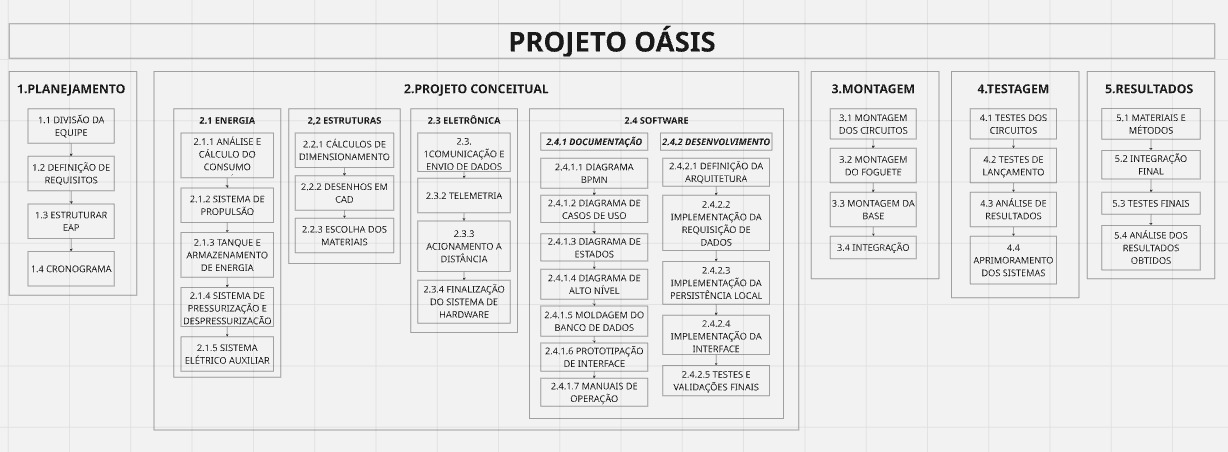
\includegraphics[width=1\linewidth]{editaveis/figuras/EAP_ProjetoOasis.jpeg}
    \caption{Estrutura analítica de projeto}
    \label{fig:enter-label}
\end{figure}

\end{landscape}


\begin{landscape}
\section{Descrição de \textit{software}}
\subsection{Diagrama BPMN}

O BPMN é uma notação que oferece modelos e representações gráficas para visualizar de forma clara os fluxos de atividades e as etapas dos processos dentro de ambientes empresariais e projetos. Seu principal foco é fornecer diagramas de fácil compreensão para todas as pessoas envolvidas, garantindo que todos os membros do grupo estejam alinhados aos objetivos do projeto.

\begin{figure}[H]
    \centering
    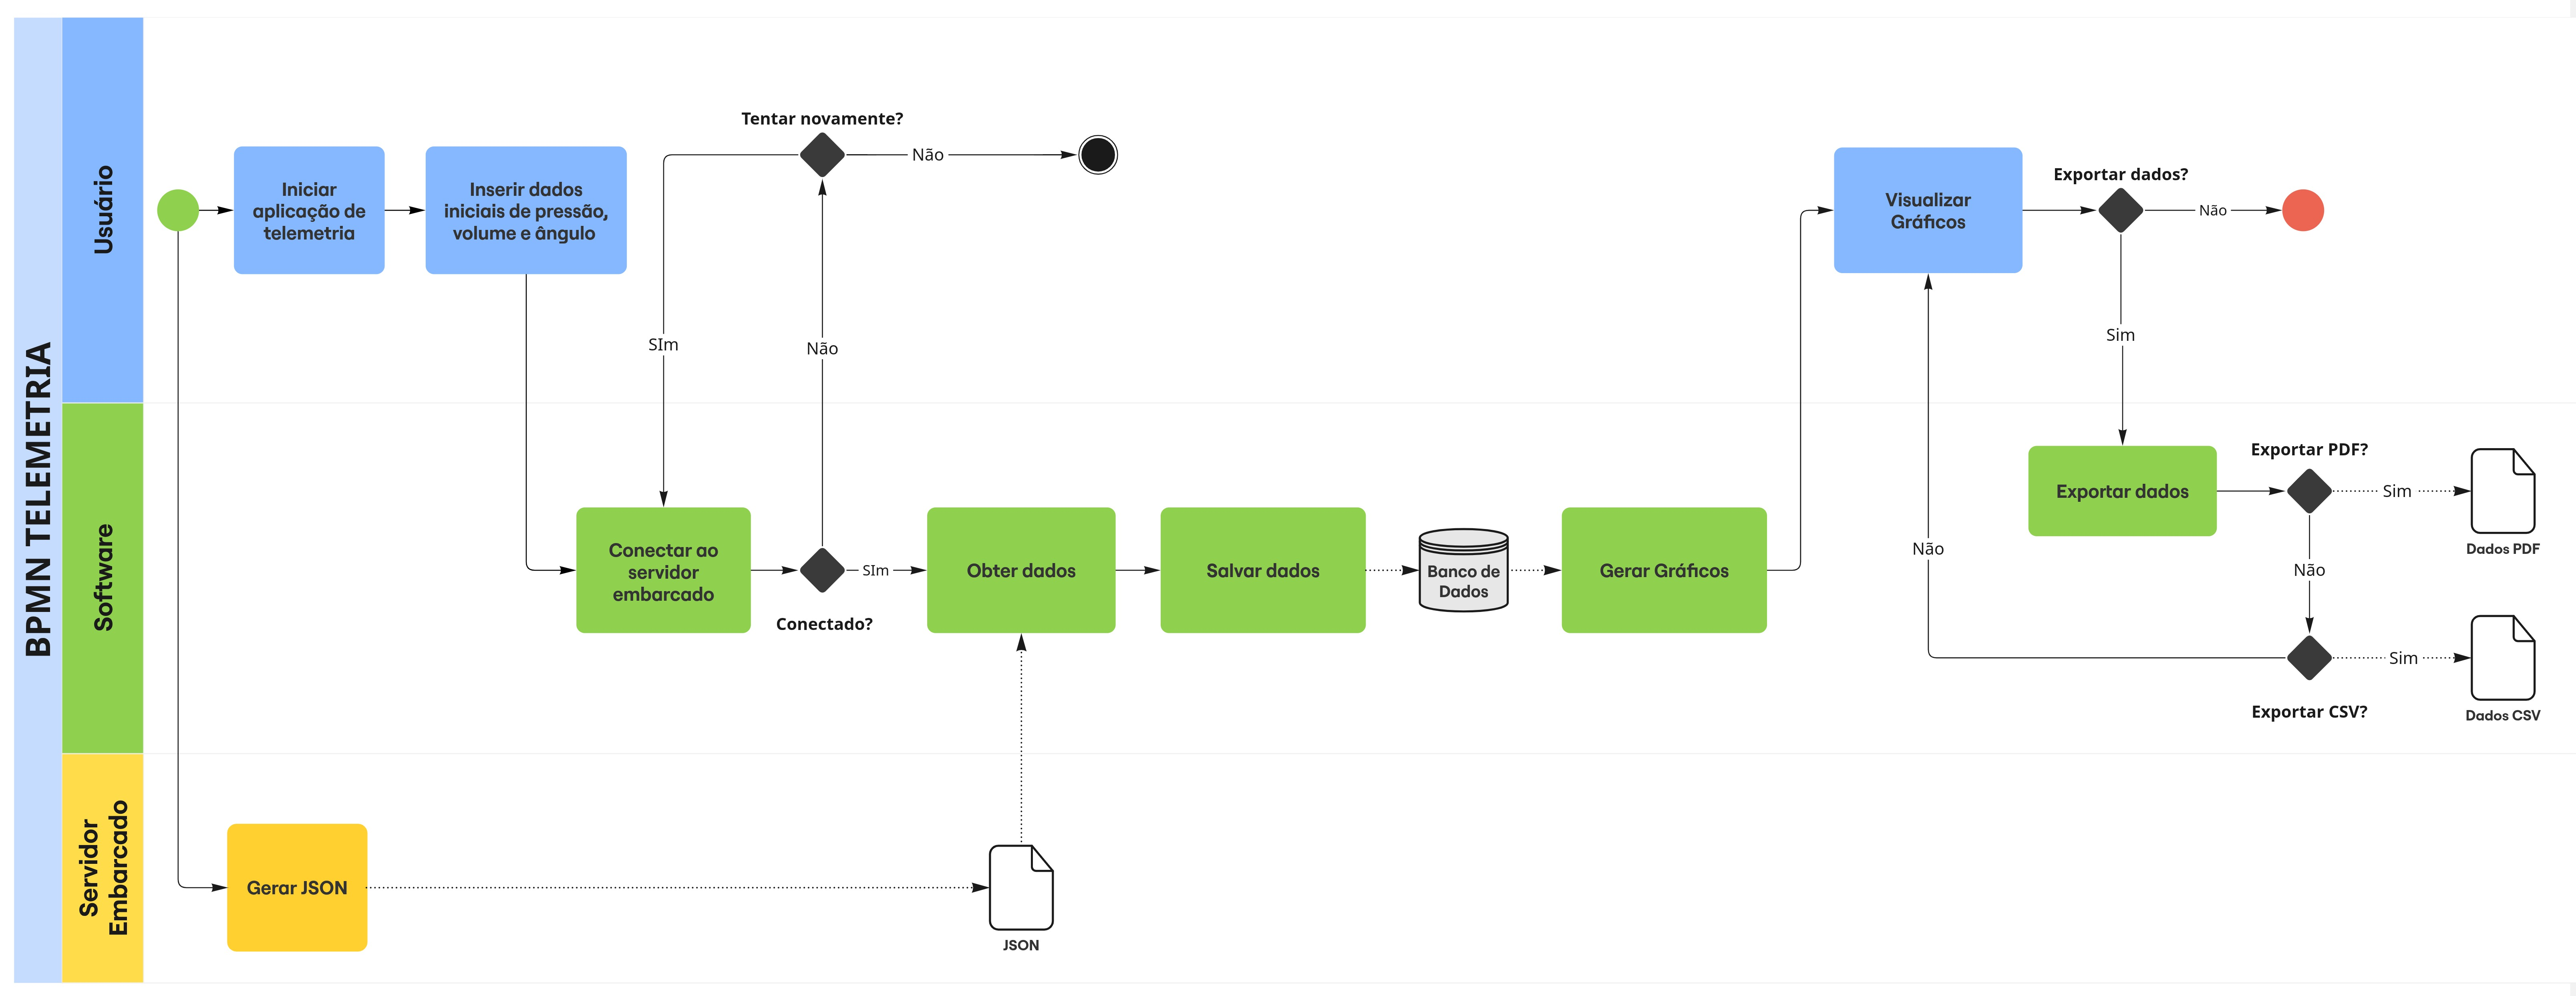
\includegraphics[width=1\linewidth]{editaveis/figuras/bpmn.jpg}
    \caption{Diagrama BPMN}
    \label{fig:enter-label}
\end{figure}
\end{landscape}

\subsection{Backlog Funcional}
O backlog funcional é uma lista organizada de funcionalidades que um sistema deve implementar para atender às necessidades dos usuários. Ele serve como um guia para o desenvolvimento do software, definindo o que precisa ser feito, por que e para quem.

O backlog funcional do projeto Oásis segue o formato de histórias de usuário, representando os requisitos funcionais sob a perspectiva do usuário final. Elas seguem um formato padrão:

\textit{“Eu, como [tipo de usuário], quero [ação] para [benefício].”}

Esse formato ajudará a equipe de software a entender quem vai usar a funcionalidade, o que a pessoa deseja fazer e por que tal funcionalidade é importante.

Os requisitos funcionas foram classificados utilizando o MoSCoW, técnica utilizada para definir a prioridade de cada funcionalidade no backlog.

O operador representa a pessoa que utilizará diretamente o sistema.

\setlength{\extrarowheight}{2pt}

\begin{longtable}{|>{\centering\arraybackslash}m{2cm}|
                    >{\centering\arraybackslash}m{2.7cm}|
                    >{\centering\arraybackslash}m{1cm}|
                    >{\centering\arraybackslash}m{6cm}|
                    >{\centering\arraybackslash}m{2cm}|}
  \hline
  \textbf{Épico} & \textbf{Feature} & \textbf{ID} & \textbf{História de Usuário} & \textbf{MoSCoW} \\
  \hline
  \endfirsthead
  
  \hline
  \textbf{Épico} & \textbf{Feature} & \textbf{ID} & \textbf{História de Usuário} & \textbf{MoSCoW} \\
  \hline
  \endhead

E01 Coleta de Telemetria
    & F01: Conexão ao servidor embarcado & US01 & Eu, como operador, quero conectar o software ao servidor embarcado no foguete para iniciar a leitura dos dados de voo. & Must \\
  \cline{2-5}
    & F02: Requisição de dados JSON & US02 & Eu, como operador, quero requisitar os dados do voo em formato JSON para processá-los no sistema. & Must \\
  \cline{2-5}
    & F03: Persistência dos dados & US03 & Eu, como operador, quero salvar os dados coletados em um banco de dados para uso posterior e comparação entre lançamentos. & Must \\
  \hline

E02 Análise de Voo
    & F04: Visualização gráfica & US04 & Eu, como operador, quero visualizar gráficos de aceleração e velocidade para analisar a trajetória do foguete. & Must \\
  \cline{2-5}
    & F05: Indicadores de desempenho & US05 & Eu, como operador, quero ver o tempo de voo e distância final para verificar se os requisitos de alcance foram atendidos. & Should \\
  \cline{2-5}
    & F06: Análise comparativa & US06 & Eu, como operador, quero comparar os dados entre os três lançamentos para calibrar o foguete com base nos resultados. & Could \\
  \hline

E03 Interface com o Usuário
    & F07: Dashboard interativo & US07 & Eu, como operador, quero navegar entre as telas de conexão, gráficos e análise para usar o sistema com facilidade. & Should \\
  \cline{2-5}
    & F08: Exportação dos dados & US08 & Eu, como operador, quero exportar os dados dos lançamentos em CSV para realizar análises externas. & Could \\
  \cline{2-5}
    & F09: Exportar relatório em PDF & US09 & Eu, como operador, quero exportar os gráficos e dados em formato .PDF para documentar o desempenho do foguete. & Could \\
  \hline

E04 Calibração de Trajetória
    & F10: Ajuste por parâmetros & US10 & Eu, como operador, quero visualizar os dados de entrada como pressão, volume e ângulo para entender seu impacto no desempenho. & Should \\
  \hline

\end{longtable}



\begin{itemize}
    \item \textcolor{red}{\textbf{ \textit{Backlog} não-funcional do \textit{software}:}}
    \begin{itemize}
        \item \textcolor{red}{ Descrever os requisitos não-funcionais de forma objetiva;}
        \item \textcolor{red}{ Mais facilmente, mais rapidamente, são descrições subjetivas não-válidas. Um exemplo de requisito não-funcional de desempenho: ``a página deve carregar em até 5s quando em conexão 4G''. }
    \end{itemize}
    \item \textcolor{red}{ \textbf{Diagrama de casos de uso,} contendo os atores do sistema, os requisitos com os quais eles interagem e os tipos de relacionamentos entre requisitos realizados por um mesmo ator (ex.: \textit{include}, \textit{extend}). Obs.: este é um diagrama sobre requisitos funcionais.}
    \item \textcolor{red}{ \textbf{Descrição da arquitetura da solução de \textit{software} proposta:}}
    \begin{itemize}
        \item \textcolor{red}{ Propósito do \textit{software} (qual o seu papel no sistema);}
        \item \textcolor{red}{ Estilo arquitetural contendo:}
        \begin{itemize}
            \item \textcolor{red}{ Padrão adotado: MVC, MVP, Microsserviços, Monolítico, etc (Justificar);}
            \item \textcolor{red}{ Linguagens de programação: Java, Python, C\#, JavaScript, etc.}
            \item \textcolor{red}{ \textit{Frameworks} e bibliotecas: Spring Boot, .NET Core, React, Angular, Django, etc.}
            \item \textcolor{red}{ Banco de dados: Relacional (PostgreSQL, MySQL, etc) X NãoSQL (MongoDB,etc). }
        \end{itemize}
        \item \textcolor{red}{ Diagrama de alto nível: representação esquemática dos componentes da arquitetura, suas responsabilidades e comunicações, esclarecendo a composição do \textit{front-end} e do \textit{back-end}.}
    \end{itemize}
    \item \textcolor{red}{ \textbf{Persistência de dados:} diagrama de entidade relacionamento do banco de dados usado na solução proposta.}
    \item \textcolor{red}{ \textbf{Análise de dados:} as variáveis definidas nos requisitos do projeto em abordagem numérica e gráfica.}
    


\subsection{Diagrama de Estados}
O diagrama de estados é um tipo de diagrama utilizado para modelar o comportamento dinâmico de um sistema, descrevendo os diferentes estados que um objeto ou sistema pode assumir ao longo do tempo, bem como os eventos ou condições que causam as transições entre esses estados.

\begin{landscape}
\begin{figure}
    \centering
    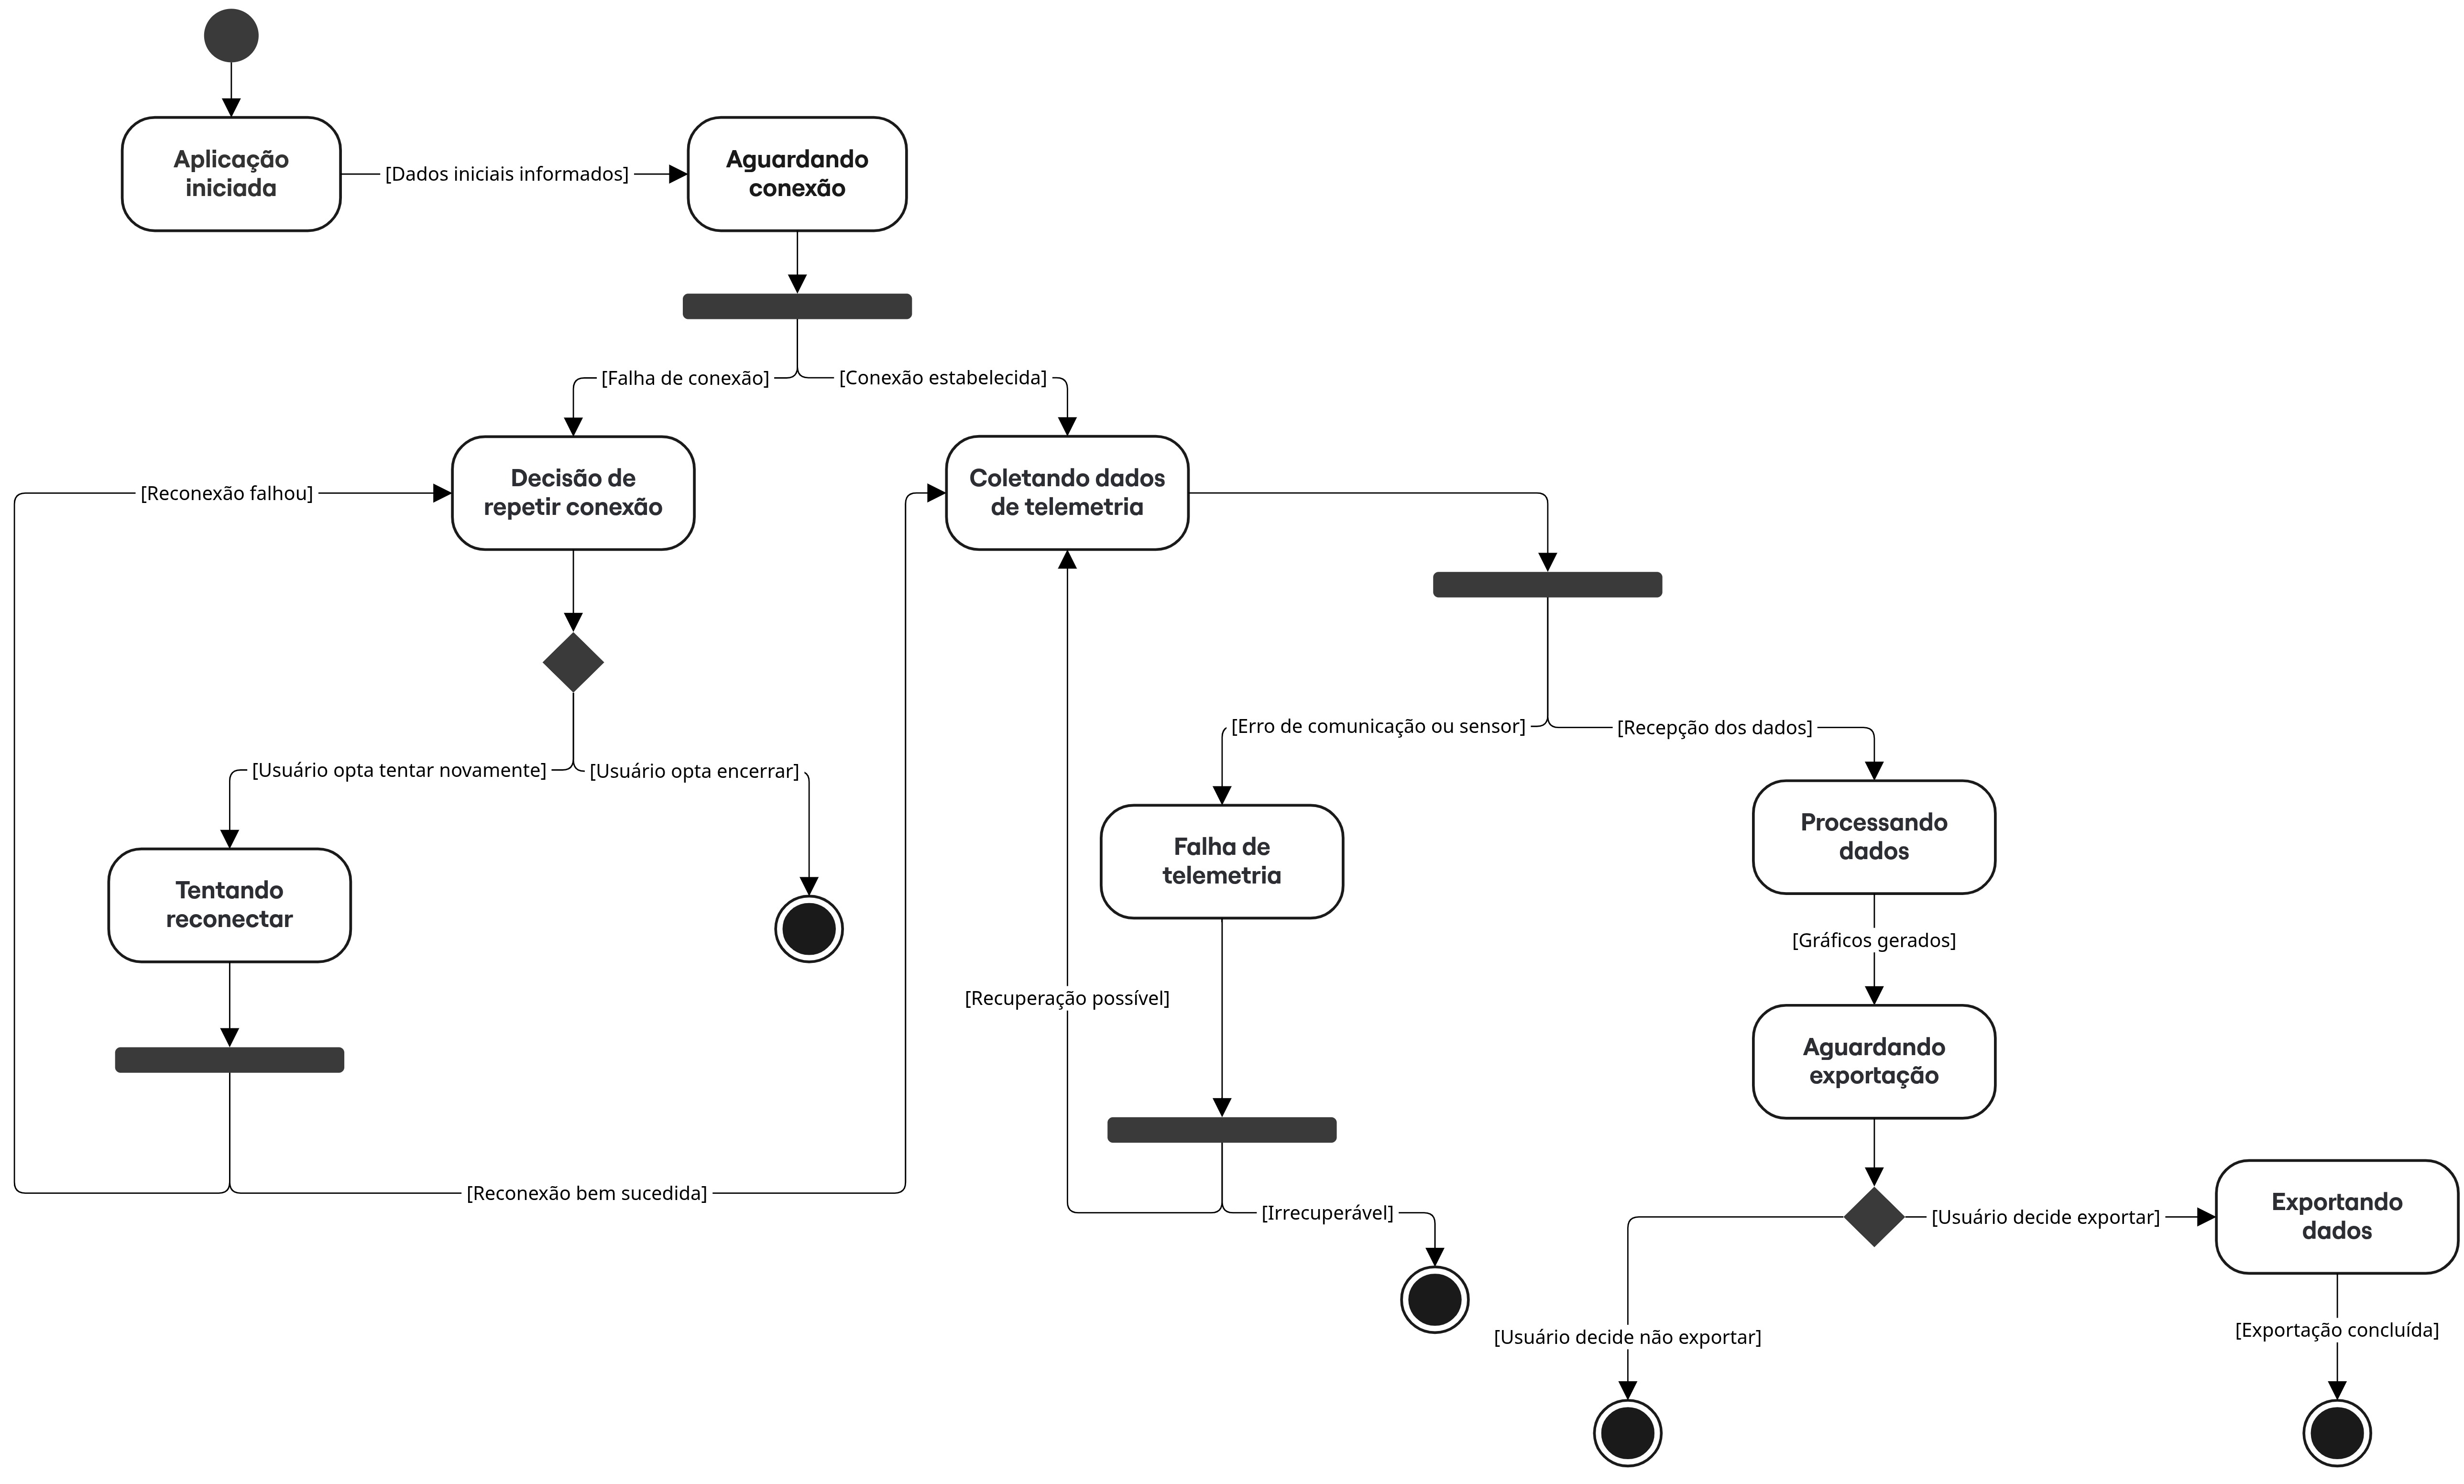
\includegraphics[width=1\linewidth]{editaveis/figuras/diagrama_de_estados.jpg}
    \caption{Diagrama de Estados}
    \label{fig:enter-label}
\end{figure}
\end{landscape}


    \item \textcolor{red}{ \textbf{Protótipo funcional do \textit{software}, navegável.}}
    \item \textcolor{red}{\textbf{ Roteiro de testes funcionais:} }
    \begin{itemize}
        \item \textcolor{red}{Código do caso de teste;}
        \item \textcolor{red}{Nome do caso de teste;}
        \item \textcolor{red}{Tipo do caso de teste (unitário, integrado ou sistema);}
        \item \textcolor{red}{ Objetivo do caso de teste;}
        \item \textcolor{red}{ Pré-condições do sistema para o teste ser realizado;}
        \item \textcolor{red}{ Descrição dos procedimentos a serem executados para o teste;}
        \item \textcolor{red}{ Resultado esperado para o teste ser aprovado (pós-condição após realizado o teste);}
        \item \textcolor{red}{ Especificação do reparo a ser executado (caso o teste não seja aprovado);}
        \item \textcolor{red}{ Resultado após reparo (o caso do teste ser necessário de ser repetido após reparo).}
    \end{itemize}
\end{itemize}


% \section{Estrutura}

% \textcolor{red}{Apresentar desenho em CAD, indicar dimensões por lado/aresta/cota, indicar materiais utilizados e explicar o desenho e as decisões de projeto.}

% \section{Descrição de \textit{hardware}}

% \textcolor{black}{A descrição de hardware deste documento foi elaborada para garantir a replicabilidade do sistema, seguindo padrões técnicos e organizacionais claros. Para isso, são apresentados três elementos fundamentais: }

% \textcolor{black}{\begin{itemize}
%     \item O diagrama de blocos \cite{blockdiagram}: Oferece uma visão geral da arquitetura, destacando a interação entre sensores, atuadores, núcleo de controle e subsistemas de alimentação, com as principais partes do sistema e as ligações entre elas.
%     \item A lista de materiais \cite{bom}: que facilita a montagem do sistema a partir da escolha dos componentes, quantidades e custos, permitindo o planejamento financeiro e a aquisição precisa de itens.
%     \item O esquemático \cite{esquematico}: Detalha as conexões físicas entre os elementos, incluindo pinagem, protocolos de comunicação e proteção de circuitos.
% \end{itemize}}

% \textcolor{black}{Além disso, as justificativas técnicas embasam as escolhas dos componentes, garantindo que cada decisão esteja alinhada com os requisitos de desempenho, segurança e custo-benefício. Essa estrutura permite não apenas a reprodução fiel do projeto, mas também sua adaptação para cenários alternativos, como a inclusão de novos sensores ou a otimização de consumo energético. }

% \section{Análise de consumo energético}

% Nessa seção, faremos a modelagem matemática do projeto, analisando objetivos, estrutura, movimento e trajetória. Nesse primeiro momento, ao analisar o movimento cinemático do foguete, utilizaremos a referência \cite{moyses}.

%  Tendo em vista o objetivo de atingir um alcance máximo de 30 metros, definimos então que num ângulo de lançamento de 45° o foguete deve atingir os 30 metros de alcance, uma vez que esse é o ângulo de alcance máximo para o lançamento de um projétil.  Analisando as componentes vertical e horizontal do movimento do foguete, vamos encontrar o tempo necessário para que ele realize o movimento completo:
% \begin{equation}
%     v=v_{oy}+\frac{at}{2} \xrightarrow{} 0=v_{oy}-\frac{9,81t}{2}\xrightarrow{}v_{oy}=\frac{9,81t}{2},
%     \label{componente vertical}
% \end{equation}
% \begin{equation}
%     s=s_o+v_{ox}.t \xrightarrow{} 30=v_{ox}.t \xrightarrow{} v_{ox}=\frac{30}{t}.
%     \label{componente horizontal}
% \end{equation}

% Note que na equação \ref{componente vertical}, o tempo t é dividido por 2, uma vez que essa componente da velocidade zera o seu valor ao chegar na altura máxima, ou seja, na metade da trajetória.

% Considerando que o ângulo de lançamento para esse caso é de 45°, as componentes \(v_{ox}\) e \(v_{oy}\) são numericamente iguais, portanto:
% \begin{equation}
%     \frac{30}{t}=\frac{9,81t}{2} \xrightarrow{} t^2=\frac{30.2}{9,81} \xrightarrow{} t \approx 2,5s.
%     \label{tempo t}
% \end{equation}

% A partir disso, encontramos, também, a velocidade inicial necessária do foguete:

% \begin{equation}
%      v_o.cos 45°=v_{ox} \xrightarrow{} v_o= \frac{v_{ox}.2}{\sqrt{2}}\xrightarrow{} v_o=\frac{\frac{30}{t}2}{\sqrt{2}} \xrightarrow{} v_o \approx 17 m/s.
%      \label{vo}
% \end{equation}

% Agora que analisamos o movimento cinemático do projeto, partimos para a dinâmica, ou seja, tudo aquilo que causa o movimento do foguete. Para esse cálculo analítico, utilizaremos a referência \cite{rocketpropulsionelements}.
% Encontramos primeiramente, a velocidade de escape da água, por meio da equação do foguete. Entretanto, são necessários os parâmetros de massa do foguete, ou seja, a massa inicial do foguete com água e a massa final dele, depois de todo o impulso dado. Para esses parâmetros faremos uma estimativa a partir dos cálculos e dados experimentais encontrados em \cite{tcc}, onde, para o nosso objetivo, a razão de massas é de aproximadamente 6. Encontramos, então, a velocidade de escape da água:
% \begin{equation}
%     \Delta V=v_o= v_e.\ln{\frac{m_o}{m_f}}.
%     \label{ve}
% \end{equation}
% \begin{equation}
%     v_e=\frac{\Delta V}{\ln{\frac{m_o}{m_f}}} \xrightarrow{} v_e=\frac{17}{ln{6}} \approx 9,5 m/s.
% \end{equation}
% Sabendo a velocidade de escape, podemos, por meio da equação de Bernoulli, considerando o fluxo ideal e incompressível e a densidade da água de 1000 \(kg/m^3\) , encontrar a pressão manométrica do foguete, ou seja, a pressão necessária dentro da cápsula de ar para o alcance da missão.

% \begin{equation}
%     P_o+\frac{\rho. v^2}{2}=P+\frac{\rho . v_e^2}{2} \xrightarrow{} \Delta P=\frac{\rho.v_e^2}{2} - \cancel{\frac{\rho.v^2}{2}} \xrightarrow{} \Delta P=\frac{1000.9,5^2}{2} \approx 45125 Pa.
%     \label{delta P}
% \end{equation}

% Calculamos, então, o fluxo de massa de água, por meio de:
% \begin{equation}
%     \dot{m}=\rho.A.v_e
%     \label{mponto}
% \end{equation}
% em que A é a área de saída da água. Estimando a área de saída da garrafa como aproximadamente 5 \(cm^2\), encontramos o seguinte resultado de fluxo de massa:
% \begin{equation}
%     \dot{m}=1000.5.10^{-4}.9,5 \approx 4,75kg/s.
% \end{equation}
% Calculamos então o empuxo necessário:
% \begin{equation}
%     T=\dot{m}.v_e=4,75.9,5=45N
%     \label{empuxo}
% \end{equation}

% Por fim, baseado na teoria proposta pela referência \cite{rocketpropulsionelements}, e considerando que o "tempo de queima", ou seja, o tempo de duração que a água vai ser expelida seja 1/10 do tempo da trajetória, encontramos o impulso total necessário:
% \begin{equation}
%     I_t=T.\Delta t =45.0,25=11,25N.s
%     \label{impulso total}
% \end{equation}

% E, finalmente, calculamos o consumo de água do foguete para um alcance de 30 metros:
% \begin{equation}
%     Q_{agua}=4,75.0,25=1,1875L .
%     \label{quantidade de agua}
% \end{equation}

% Para os outros alcances, vamos variar apenas a pressão necessária no compartimento, ou seja, manteremos o ângulo de lançamento. Repetimos o processo dos cálculos para um alcance de 10 m e 20 m.


% \begin{table}[h!]
% \centering
% \begin{tabular}{llllllllll}
% Alcance & t & $t_q$ & $v_o$ & $v_e$ & $\dot{m}$ & T & $I_t$ & $\Delta P$ & $Q_{agua}$ \\
% 10m & 1,45s & 0,145s & $9,75m/s$ & $5,45m/s$ & $2,72kg/s$ & 14,8N & 2,15N.s & 14851Pa & 0,4L \\
% 20m & 2,04s & 0,204s & $13,86m/s$ & $7,75m/s$ & $3,88kg/s$ & 30N & 6,12N.s & 30031Pa & 0,8L
% \end{tabular}
% \end{table}


% Foi feito o mesmo passo a passo das contas feitas para um alcance de 30 metros, considerando \(t_q\) o suposto "tempo de queima", utilizando as seguintes equações: equação \ref{tempo t} para o tempo t, equação \ref{vo} para o \(v_o\), equação \ref{ve} para o cálculo do \(v_e\), equação \ref{mponto} para o cálculo do \(\dot{m}\), equação \ref{empuxo} para o cálculo de T, equação \ref{impulso total} para o cálculo do \(I_t\), equação \ref{delta P} para o cálculo do \(\Delta P\) e, por fim, equação \ref{quantidade de agua} para o cálculo do \(Q_{agua}\).

% Para garantir o funcionamento eficiente do sistema eletrônico no foguete de água, é fundamental realizar uma análise do consumo energético. 	Como o projeto envolve diversos componentes eletrônicos com exigências distintas de tensão e corrente, será utilizado um regulador de tensão. Esse dispositivo permitirá adaptar a tensão fornecida pela bateria às necessidades específicas de cada parte do circuito, assegurando a integridade e o desempenho ideal. 

% Para  analisar a potência consumida em cada componente individualmente, será considerado o consumo médio da corrente e a tensão ideal. A forma utilizada para o cálculo é:
% \begin{equation}
%     P = V \cdot I 
% \end{equation}

% onde P é a potência (em watts), V é a tensão (em volts), e I a corrente elétrica (em amperes)

% A partir dos dados obtidos, será possível estimar o consumo total do sistema e, com isso, selecionar uma bateria que ofereça a tensão adequada e capacidade suficiente para garantir a autonomia e o funcionamento seguro durante toda a operação do foguete.

% \begin{figure}[H]
%     \centering
%     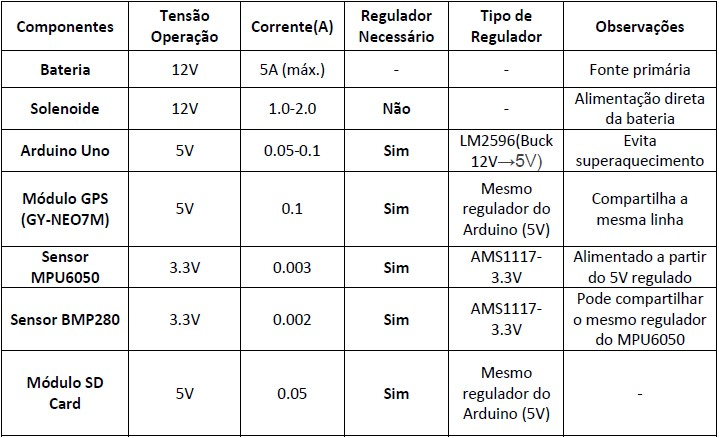
\includegraphics[width=0.75\textwidth]{figuras/Tabela.jpg}
%     \label{fig:tabela}
% \end{figure}

% \noindent Esquema de Conexões:

% \begin{figure}[H]
%     \centering
%     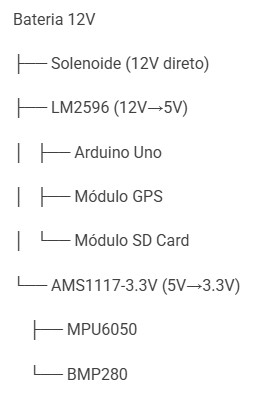
\includegraphics[width=0.3\textwidth]{figuras/Esquema.jpg}
%     \label{fig:tabela}
% \end{figure}


% \noindent Cálculo de autonomia:
% \begin{itemize}
%     \item Energia da Bateria
%     \item $12V \cdot5Ah = 60 Wh (216.000J)$
%     \item Consumo por lançamento: ~242J (incluindo solenoide)
%     \item Lançamentos possíveis:
% \end{itemize}
% \quad \qquad 216.000J/242J/lançamento = 216.000J $\approx$ 892 lançamentos



% \section{Descrição de \textit{software}}

% \textcolor{red}{Com relação ao \textit{software}, será necessário apresentar os seguintes itens: % pacotes de componentes de \textit{software}, suas funções e características, e explicar as decisões de projeto:
% \begin{enumerate}
%     \item Um diagrama do processo de negócio do problema que a máquina se propõe a resolver (BPNM) – não é UML, mas é fundamental para entender como o sistema se comporta como um todo, incluindo o usuário;
%     \item Lista de casos de uso (backlog do sistema). Backlog funcional;
%     \item Lista de requisitos não-funcionais a serem satisfeitos pelo sistema;
%     \item Diagrama de casos de uso: mostrando os requisitos funcionais, seus atores e como eles interagem entre si;
%     \item Diagrama de Classes: apresentando quais dados são manipulados pelo sistema (internamente e externamente – ex.: resultados de experimentos);
%     \item Diagrama de arquitetura, identificando todos os componentes da máquina e suas iterações com o software;
%     \item Diagrama de estados da máquina (sistema);
%     \item Descrição dos testes dos componentes da máquina e dos testes funcionais que deveriam ser feitos para avaliar o funcionamento da máquina e identificar defeitos. São importantes os testes unitários (componentes) e de integração (conjunto de componentes) e o roteiro de testes.
% \end{enumerate}
% }
% %\textcolor{red}{Com relação ao \textit{software}, será necessário apresentar pacotes de componentes de \textit{software}, suas funções e características, e explicar as decisões de projeto.}


\input{editaveis/07_orcamento}
%\begin{landscape}

\chapter{Cronograma do projeto}

\begin{table}[htpb]
\begin{center}
\caption{Cronograma geral.}
\begin{tabular}{|c|c|c|}
\hline
\textbf{Geral}          & \textbf{Previsto} & \textbf{Realizado} \\ \hline
Início do projeto  & 16/04/2025 & 16/04/2025         \\ \hline
Fim do projeto   & 16/07/2025 &         \\ \hline
\end{tabular}
\end{center}
\end{table}

\begin{landscape}

\begin{table}[htpb]
\begin{center}
\caption{Cronograma por atividade.}
\begin{tabular}{|c|c|c|c|c|c|c|}
\hline
& \textbf{Início} & \textbf{Início} & \textbf{Fim} & \textbf{Fim} & \textbf{Atividades} & \\
\textbf{Atividade} & \textbf{Previsto} & \textbf{Realizado} & \textbf{Previsto} & \textbf{Realizado} & \textbf{Predecessoras} & \textbf{Responsáveis}\\ \hline

1- Planejamento e definição do cronograma  & 16/04/2025      & 16/04/2025 & 25/04/2025 & 25/04/2025 & - & Gerência geral  
\\ \hline

2- Cálculo de consumo energético & 20/04/2025 & 20/04/2025 & 01/06/2025 & 02/06/2025 & 1 & Energia 
\\ \hline

3- Cálculos de trajetória & 06/05/2025 & 06/05/2025 & 01/06/2025 & 02/06/2025 & 1 & Estruturas 
\\ \hline

4- Testes e definição de Hardware & 10/05/2025 & 10/05/2025 & 28/05/2025 & 28/05/2025 & 1 & Eletrônica     \\ \hline

5- Diagrama BPMN e Backlog Funcional & 12/05/2025 & 17/05/2025 & 17/05/2025 & 17/05/2025 & 1 & Software       \\ \hline

6- Backlog Não-Funcional & 13/05/2025 & 17/05/2025 & 17/05/2025 & 17/05/2025 & 1 & Software 
\\ \hline

7- Diagrama de Casos de Uso (UML) & 13/05/2025 & 17/05/2025 & 18/05/2025 & 18/05/2025 & 1 & Software        \\ \hline

8- Descrição da Arquitetura de Software & 15/05/2025 & 26/05/2025 & 22/05/2025 & 26/05/2025 & 5, 6 e 7 & Software 
\\ \hline

9- Diagrama ER (Entidade-Relacionamento) & 15/05/2025 & 21/05/2025 & 22/05/2025 & 21/05/2025 & 1 & Software       \\ \hline

10- Diagrama de Estados (UML) & 19/05/2025 & 25/05/2025 & 25/05/2025 & 25/05/2025 & 1 & Software              
\\ \hline

11- Desenhos técnicos & 19/05/2025 & 27/05/2025 & 26/05/2025 & 01/06/2025 & 3 & Estruturas            
\\ \hline

12- Escolha dos materiais & 19/05/2025 & 19/05/2025 & 26/05/2025 & 02/06/2025 & 3 & Estruturas            
\\ \hline

13- Construção do foguete e da base & 27/05/2025 & 21/05/2025 & 09/06/2025 &  & 11 e 12 & Estruturas         \\ \hline

14- Análise de Dados & 20/05/2025 & 21/05/2025 & 26/05/2025 & 21/05/2025 & 9 & Software              
\\ \hline

15- Protótipo Funcional Navegável & 22/05/2025 & 31/05/2025 & 27/05/2025 & 31/05/2025 & 8 e 9 & Software   \\ \hline

16- Roteiro de Testes Funcionais & 23/05/2025 & 28/05/2028 & 28/05/2028 & 28/05/2028 & 8 e 9 & Software
\\ \hline

17- Testes de lançamento & 27/05/2025 & 28/05/2025 & 15/06/2025 &  & 13 & Estruturas            
\\ \hline

18- Montagem e testes iniciais de Hardware & 29/05/2025 & 29/05/2025 & 07/06/2025 & 07/06/2025 & 4 & Eletrônica 
\\ \hline

19- Análise de resultados de lançamento & 30/05/2025 & 28/05/2025 & 17/05/2025 &   & 17 & Todos                 \\ \hline
20- Integração dos sistemas & 10/06/2025 &  & 20/06/2025 &  & 1-19 & Todos
\\ \hline              

\end{tabular}
\end{center}
\end{table}



%\begin{table}[htpb]
%\begin{center}
%\caption{Justificativas para atrasos ou não-conclusão de atividades.}
% \begin{tabular}{|c|c|} \hline
% \textbf{Atividade} & \textbf{Justificativa}  \\ \hline 
%     3 - GHI &
%     O material solicitado não foi entregue no prazo pelo fornecedor. \\ \hline
%     5 - MNO &
%     A equipe responsável pelo desenvolvimento não finalizou a atividade. \\ \hline
% \end{tabular}
% \end{center}
% \end{table}



%%% Exemplo de tabela que ocupa várias páginas
% \begin{center}
% \begin{longtable}{|l|l|l|}
% \caption{A sample long table.} \label{tab:long} \\

% \hline \multicolumn{1}{|c|}{\textbf{First column}} & \multicolumn{1}{c|}{\textbf{Second column}} & \multicolumn{1}{c|}{\textbf{Third column}} \\ \hline 
% \endfirsthead

% \multicolumn{3}{c}%
% {{\bfseries \tablename\ \thetable{} -- continued from previous page}} \\
% \hline \multicolumn{1}{|c|}{\textbf{First column}} & \multicolumn{1}{c|}{\textbf{Second column}} & \multicolumn{1}{c|}{\textbf{Third column}} \\ \hline 
% \endhead

% \hline \multicolumn{3}{|r|}{{Continued on next page}} \\ \hline
% \endfoot

% \hline \hline
% \endlastfoot

% One & abcdef ghjijklmn & 123.456778 \\
% One & abcdef ghjijklmn & 123.456778 \\
% One & abcdef ghjijklmn & 123.456778 \\
% One & abcdef ghjijklmn & 123.456778 \\
% One & abcdef ghjijklmn & 123.456778 \\
% One & abcdef ghjijklmn & 123.456778 \\
% One & abcdef ghjijklmn & 123.456778 \\
% One & abcdef ghjijklmn & 123.456778 \\
% One & abcdef ghjijklmn & 123.456778 \\
% One & abcdef ghjijklmn & 123.456778 \\
% One & abcdef ghjijklmn & 123.456778 \\
% One & abcdef ghjijklmn & 123.456778 \\
% One & abcdef ghjijklmn & 123.456778 \\
% One & abcdef ghjijklmn & 123.456778 \\
% One & abcdef ghjijklmn & 123.456778 \\
% One & abcdef ghjijklmn & 123.456778 \\
% One & abcdef ghjijklmn & 123.456778 \\
% One & abcdef ghjijklmn & 123.456778 \\
% One & abcdef ghjijklmn & 123.456778 \\
% One & abcdef ghjijklmn & 123.456778 \\
% One & abcdef ghjijklmn & 123.456778 \\
% One & abcdef ghjijklmn & 123.456778 \\
% One & abcdef ghjijklmn & 123.456778 \\
% One & abcdef ghjijklmn & 123.456778 \\
% One & abcdef ghjijklmn & 123.456778 \\
% One & abcdef ghjijklmn & 123.456778 \\
% One & abcdef ghjijklmn & 123.456778 \\
% One & abcdef ghjijklmn & 123.456778 \\
% One & abcdef ghjijklmn & 123.456778 \\
% One & abcdef ghjijklmn & 123.456778 \\
% One & abcdef ghjijklmn & 123.456778 \\
% One & abcdef ghjijklmn & 123.456778 \\
% One & abcdef ghjijklmn & 123.456778 \\
% One & abcdef ghjijklmn & 123.456778 \\
% One & abcdef ghjijklmn & 123.456778 \\
% One & abcdef ghjijklmn & 123.456778 \\
% \end{longtable}
% \end{center}

\end{landscape}
\input{editaveis/09_resultados}
\input{editaveis/10_licoes}

% \part{Aspectos Gerais}

\chapter[Aspectos Gerais]{Aspectos Gerais}

Estas instruções apresentam um conjunto mínimo de exigências necessárias a 
uniformidade de apresentação do relatório de Trabalho de Conclusão de Curso 
da FGA. Estilo, concisão e clareza ficam inteiramente sob a 
responsabilidade do(s) aluno(s) autor(es) do relatório.

As disciplinas de Trabalho de Conclusão de Curso (TCC) 01 e Trabalho de 
Conclusão de Curso (TCC) 02 se desenvolvem de acordo com Regulamento 
próprio aprovado pelo Colegiado da FGA. Os alunos matriculados nessas 
disciplinas devem estar plenamente cientes de tal Regulamento. 

\section{Composição e estrutura do trabalho}

A formatação do trabalho como um todo considera três elementos principais: 
(1) pré-textuais, (2) textuais e (3) pós-textuais. Cada um destes, pode se 
subdividir em outros elementos formando a estrutura global do trabalho, 
conforme abaixo (as entradas itálico são \textit{opcionais}; em itálico e
negrito são \textbf{\textit{essenciais}}):

\begin{description}
	\item [Pré-textuais] \

	\begin{itemize}
		\item Capa
		\item Folha de rosto
		\item \textit{Dedicatória}
		\item \textit{Agradecimentos}
		\item \textit{Epígrafe}
		\item Resumo
		\item Abstract
		\item Lista de figuras
		\item Lista de tabelas
		\item Lista de símbolos e
		\item Sumário
	\end{itemize}

	\item [Textuais] \

	\begin{itemize}
		\item \textbf{\textit{Introdução}}
		\item \textbf{\textit{Desenvolvimento}}
		\item \textbf{\textit{Conclusões}}
	\end{itemize}

	\item [Pós-Textuais] \
	
	\begin{itemize}
		\item Referências bibliográficas
		\item \textit{Bibliografia}
		\item Anexos
		\item Contracapa
	\end{itemize}
\end{description}

Os aspectos específicos da formatação de cada uma dessas três partes 
principais do relatório são tratados nos capítulos e seções seguintes.

No modelo \LaTeX, os arquivos correspondentes a estas estruturas que devem
ser editados manualmente estão na pasta \textbf{editáveis}. Os arquivos
da pasta \textbf{fixos} tratam os elementos que não necessitam de 
edição direta, e devem ser deixados como estão na grande maioria dos casos.

\section{Considerações sobre formatação básica do relatório}

A seguir são apresentadas as orientações básicas sobre a formatação do
documento. O modelo \LaTeX\ \textbf{já configura todas estas opções corretamente},
de modo que para os usuários deste modelo o texto de toda esta Seção é 
\textbf{meramente informativo}.

\subsection{Tipo de papel, fonte e margens}

Papel -- Na confecção do relatório deverá ser empregado papel branco no 
formato padrão A4 (21 cm x 29,7cm), com 75 a 90 g/m2.

Fonte -- Deve-se utilizar as fontes Arial ou Times New Roman no tamanho 12 
pra corpo do texto, com variações para tamanho 10 permitidas para a 
wpaginação, legendas e notas de rodapé. Em citações diretas de mais de três 
linhas utilizar a fonte tamanho 10, sem itálicos, negritos ou aspas. Os 
tipos itálicos são usados para nomes científicos e expressões estrangeiras, 
exceto expressões latinas.

Margens -- As margens delimitando a região na qual todo o texto deverá estar 
contido serão as seguintes: 

\begin{itemize}
	\item Esquerda: 03 cm;
	\item Direita	: 02 cm;
	\item Superior: 03 cm;
	\item Inferior: 02 cm. 
\end{itemize}

\subsection{Numeração de Páginas}

A contagem sequencial para a numeração de páginas começa a partir da 
primeira folha do trabalho que é a Folha de Rosto, contudo a numeração em 
si só deve ser iniciada a partir da primeira folha dos elementos textuais. 
Assim, as páginas dos elementos pré-textuais contam, mas não são numeradas 
e os números de página aparecem a partir da primeira folha dos elementos 
textuais, que se iniciam na Introdução. 

Os números devem estar em algarismos arábicos (fonte Times ou Arial 10) no 
canto superior direito da folha, a 02 cm da borda superior, sem traços, 
pontos ou parênteses. 

A paginação de Apêndices e Anexos deve ser contínua, dando seguimento ao 
texto principal.

\subsection{Espaços e alinhamento}

Para a monografia de TCC 01 e 02 o espaço entrelinhas do corpo do texto 
deve ser de 1,5 cm, exceto RESUMO, CITAÇÔES de mais de três linhas, NOTAS 
de rodapé, LEGENDAS e REFERÊNCIAS que devem possuir espaçamento simples. 
Ainda, ao se iniciar a primeira linha de cada novo parágrafo se deve 
tabular a distância de 1,25 cm da margem esquerda.

Quanto aos títulos das seções primárias da monografia, estes devem começar 
na parte superior da folha e separados do texto que o sucede, por um espaço 
de 1,5 cm entrelinhas, assim como os títulos das seções secundárias, 
terciárias. 

A formatação de alinhamento deve ser justificado, de modo que o texto fique 
alinhado uniformemente ao longo das margens esquerda e direita, exceto para 
CITAÇÕES de mais de três linhas que devem ser alinhadas a 04 cm da margem 
esquerda e REFERÊNCIAS que são alinhadas somente à margem esquerda do texto 
diferenciando cada referência.

\subsection{Quebra de Capítulos e Aproveitamento de Páginas}

Cada seção ou capítulo deverá começar numa nova pagina (recomenda-se que 
para texto muito longos o autor divida seu documento em mais de um arquivo 
eletrônico). 

Caso a última pagina de um capitulo tenha apenas um número reduzido de 
linhas (digamos 2 ou 3), verificar a possibilidade de modificar o texto 
(sem prejuízo do conteúdo e obedecendo as normas aqui colocadas) para 
evitar a ocorrência de uma página pouco aproveitada.

Ainda com respeito ao preenchimento das páginas, este deve ser otimizado, 
evitando-se espaços vazios desnecessários. 

Caso as dimensões de uma figura ou tabela impeçam que a mesma seja 
posicionada ao final de uma página, o deslocamento para a página seguinte 
não deve acarretar um vazio na pagina anterior. Para evitar tal ocorrência, 
deve-se reposicionar os blocos de texto para o preenchimento de vazios. 

Tabelas e figuras devem, sempre que possível, utilizar o espaço disponível 
da página evitando-se a \lq\lq quebra\rq\rq\ da figura ou tabela. 

\section{Cópias}

Nas versões do relatório para revisão da Banca Examinadora em TCC1 e TCC2, 
o aluno deve apresentar na Secretaria da FGA, uma cópia para cada membro da 
Banca Examinadora.

Após a aprovação em TCC2, o aluno deverá obrigatoriamente apresentar a 
versão final de seu trabalho à Secretaria da FGA na seguinte forma:

\begin{itemize}
	\item 01 cópia encadernada para arquivo na FGA;
	\item 01 cópia não encadernada (folhas avulsas) para arquivo na FGA;
	\item 01 cópia em CD de todos os arquivos empregados no trabalho.
\end{itemize}

A cópia em CD deve conter, além do texto, todos os arquivos dos quais se 
originaram os gráficos (excel, etc.) e figuras (jpg, bmp, gif, etc.) 
contidos no trabalho. Caso o trabalho tenha gerado códigos fontes e 
arquivos para aplicações especificas (programas em Fortran, C, Matlab, 
etc.) estes deverão também ser gravados em CD. 

O autor deverá certificar a não ocorrência de “vírus” no CD entregue a 
secretaria. 


% \chapter[Considerações sobre os Elementos Textuais]{Considerações sobre os 
Elementos Textuais}

\section{Introdução}

A regra mais rígida com respeito a Introdução é que a mesma, que é 
necessariamente parte integrante do texto, não deverá fazer agradecimentos 
a pessoas ou instituições nem comentários pessoais do autor atinentes à 
escolha ou à relevância do tema.

A Introdução obedece a critérios do Método Cientifico e a exigências 
didáticas. Na Introdução o leitor deve ser colocado dentro do espírito do 
trabalho.

Cabe mencionar que a Introdução de um trabalho pode, pelo menos em parte, 
ser escrita com grande vantagem uma vez concluído o trabalho (ou o 
Desenvolvimento e as Conclusões terem sido redigidos). Não só a pesquisa 
costuma modificar-se durante a execução, mas também, ao fim do trabalho, o 
autor tem melhor perspectiva ou visão de conjunto.

Por seu caráter didático, a Introdução deve, ao seu primeiro parágrafo, 
sugerir o mais claramente possível o que pretende o autor. Em seguida deve 
procurar situar o problema a ser examinado em relação ao desenvolvimento 
científico e técnico do momento. Assim sendo, sempre que pertinente, os 
seguintes pontos devem ser abordados: 

\begin{itemize}

	\item Contextualização ou apresentação do tema em linhas gerais de 
	forma clara e objetiva;
	\item Apresentação da justificativa e/ou relevância do tema escolhido;
	\item Apresentação da questão ou problema de pesquisa;
	\item Declaração dos objetivos, gerais e específicos do trabalho;
	\item Apresentação resumida da metodologia, e
	\item Indicação de como o trabalho estará organizado.

\end{itemize}

\section{Desenvolvimento}

O Desenvolvimento (Miolo ou Corpo do Trabalho) é subdividido em seções de 
acordo com o planejamento do autor. As seções primárias são aquelas que 
resultam da primeira divisão do texto do documento, geralmente 
correspondendo a divisão em capítulos. Seções secundárias, terciárias, 
etc., são aquelas que resultam da divisão do texto de uma seção primária, 
secundária, terciária, etc., respectivamente.

As seções primárias são numeradas consecutivamente, seguindo a série 
natural de números inteiros, a partir de 1, pela ordem de sua sucessão no 
documento.

O Desenvolvimento é a seção mais importante do trabalho, por isso exigi-se 
organização, objetividade e clareza. É conveniente dividi-lo em pelo menos 
três partes:

\begin{itemize}

	\item Referencial teórico, que corresponde a uma análise dos trabalhos 
	relevantes, encontrados na pesquisa bibliográfica sobre o assunto. 
	\item Metodologia, que é a descrição de todos os passos metodológicos 
	utilizados no trabalho. Sugere-se que se enfatize especialmente em (1) 
	População ou Sujeitos da pesquisa, (2) Materiais e equipamentos 
	utilizados e (3) Procedimentos de coleta de dados.
	\item Resultados, Discussão dos resultados e Conclusões, que é onde se 
	apresenta os dados encontrados a análise feita pelo autor à luz do 
	Referencial teórico e as Conclusões.

\end{itemize}

\section{Uso de editores de texto}

O uso de programas de edição eletrônica de textos é de livre escolha do autor. 


% \part{Texto e Pós Texto}

% \chapter[Elementos do Texto]{Elementos do Texto}

\section{Corpo do Texto}

O estilo de redação deve atentar a boa prática da linguagem técnica. Para a 
terminologia metrological usar o Vocabulário Internacional de Termos 
Fundamentais e Gerais de Metrologia \cite{inmetro2003}.

Grandezas dimensionais devem ser apresentadas em unidades consistentes com 
o Sistema Internacional de Unidades  (SI). Outras unidades podem ser usadas 
como unidades secundárias entre parenteses se necessário. Exceções são 
relacionadas a unidades não-SI usadas como identificadores comerciais como 
pro exemplo \lq\lq disquete de  3$\nicefrac{1}{2}$ polegadas\rq\rq. 

Na apresentação de números ao longo do texto usar virgula para separar a 
parte decimal de um número. Resultados experimentais devem ser apresentados 
com sua respectiva incerteza de medição.

\section{Títulos de capítulos e seções}

Recomendações de formatação de seções (texto informativo: o \LaTeX\
\textbf{já formata as seções automaticamente, se utilizado o comando
\texttt{\textbackslash section\{Nome da Seção\}}}):

\begin{description}

	\item \textbf{1 SEÇÃO PRIMÁRIA - MAIÚSCULAS; NEGRITO; TAMANHO 12;}

	\item 1.1 SEÇÃO SECUNDÁRIA – MAIÚSCULAS; NORMAL; TAMANHO 12; 

	\item \textbf{1.1.1 Seção terciária - Minúsculas, com exceção da 
	primeira letra; negrito; tamanho 12;}

	\item 1.1.1.1 Seção quaternária - Minúsculas, com exceção da primeira 
	letra; normal tamanho 12; 

 	\item \textit{1.1.1.1.1 Seção quinária - Minúsculas, com exceção da 
	primeira letra; itálico; tamanho 12.}

\end{description}

\section{Notas de rodapé}

Notas eventualmente necessárias devem ser numeradas de forma seqüencial ao 
longo do texto no formato 1, 2, 3... sendo posicionadas no rodapé de cada 
página na qual a nota é utilizada.\footnote{Como, por exemplo, esta nota. O \LaTeX\ tomará conta da numeração automaticamente.}

\section{Equações}

Equações matemáticas devem ser numeradas seqüencialmente e alinhadas a 
esquerda com recuo de 0,6 cm. Usar numerais arábicos entre parênteses, 
alinhado a direita, no formato Times New Roman de 9 pts. para numerara as 
equações como mostrado na Eq. \ref{eqn01} (novamente, o \LaTeX\ formata as
equações automaticamente).

Referências a equações no corpo do texto devem ser feitas como \lq\lq Eq. 
\ref{eqn01}\rq\rq\ quando no meio de uma frase ou como \lq\lq Equação 
\ref{eqn01}\rq\rq\ quando no inicio de uma sentença. Um espaçamento de 11 
pontos deve ser deixado acima, abaixo e entre equações subseqüentes. Para uma 
apresentação compacta das equações deve-se usar os símbolos e expressões 
matemáticos mais adequados e parênteses para evitar ambigüidades em 
denominadores. Os símbolos usados nas equações citados no texto devem 
apresentar exatamente a mesma formatação usada nas equações.
\begin{equation}
\label{eqn01}
	\frac{d\mathbf{C}}{dw} = \frac{du}{dw}\cdot \mathbf{F}_u + 
		\frac{dv}{dw}\cdot \mathbf{F}_v 
\end{equation}

O significado de todos os símbolos mostrados nas equações deve ser apresentado 
na lista de símbolos no inicio do trabalho, embora, em certas circunstancias o 
autor possa para maior clareza descrever o significado de certos símbolos no 
corpo do texto, logo após a equação.

Se uma equação aparecer no meio do parágrafo, como esta
\begin{equation}
x^n + y^n = z^n,
\end{equation}
onde $x, y, z, n \in \mathbf{N}$, o texto subsequente faz parte do parágrafo e 
não deve ser identado.

\section{Figuras e Gráficos}

As figuras devem ser centradas entre margens e identificadas por uma legenda 
alinhada a esquerda com recuo especial de deslocamento de 1,8 cm, com mostrado 
na Fig. (\ref{fig01}). O tamanho das fontes empregadas nos rótulos e anotações 
usadas nas figuras deve ser compatível com o usado no corpo do texto. Rótulos e 
anotações devem estar em português, com todas as grandezas mostradas em 
unidades do SI (Sistema Internacional de unidades) (mais uma vez, o \LaTeX\
cuidará dos aspectos de formatação e fonte das figuras).

Todas as figuras, gráficos e fotografias devem ser numeradas e referidas no 
corpo do texto adotando uma numeração seqüencial de identificação. As figuras e 
gráficos devem ser claras e com qualidade adequada para eventual reprodução 
posterior tanto em cores quanto em preto-e-branco.

As abscissas e ordenadas de todos os gráficos devem ser rotuladas com seus 
respectivos títulos em português seguida da unidade no SI que caracteriza a 
grandes entre colchetes. 

A referência explícita no texto à uma figura deve ser feita como 
\lq\lq Fig. \ref{fig01}\rq\rq\ quando no meio de uma frase ou como 
\lq\lq Figura \ref{fig01}\rq\rq\ quando no início da mesma. Referencias 
implícitas a uma dada figura devem ser feitas entre parênteses como 
(Fig. \ref{fig01}). Para referências a mais de uma figura as mesmas regras 
devem ser aplicadas usando-se o plural adequadamente. Exemplos:

\begin{itemize}
	\item \lq\lq Após os ensaios experimentais, foram obtidos os resultados 
	mostrados na Fig. \ref{fig01}, que ...\rq\rq
	\item \lq\lq A Figura \ref{fig01} apresenta os resultados obtidos, onde 
	pode-se observar que ...\rq\rq
	\item \lq\lq As Figuras 1 a 3 apresentam os resultados obtidos, 
	...\rq\rq
	\item \lq\lq Verificou-se uma forte dependência entre as variáveis citadas 
	(Fig. \ref{fig01}), comprovando ...\rq\rq
\end{itemize}

Cada figura deve ser posicionada o mais próxima possível da primeira citação 
feita à mesma no texto, imediatamente após o parágrafo no qual é feita tal 
citação, se possível, na mesma página. Em \LaTeX\, o comando \texttt{\textbackslash label} deve suceder o comando \texttt{\textbackslash caption} para que as referências às figuras fiquem com a numeração correta.
\begin{figure}[h]
	\centering
	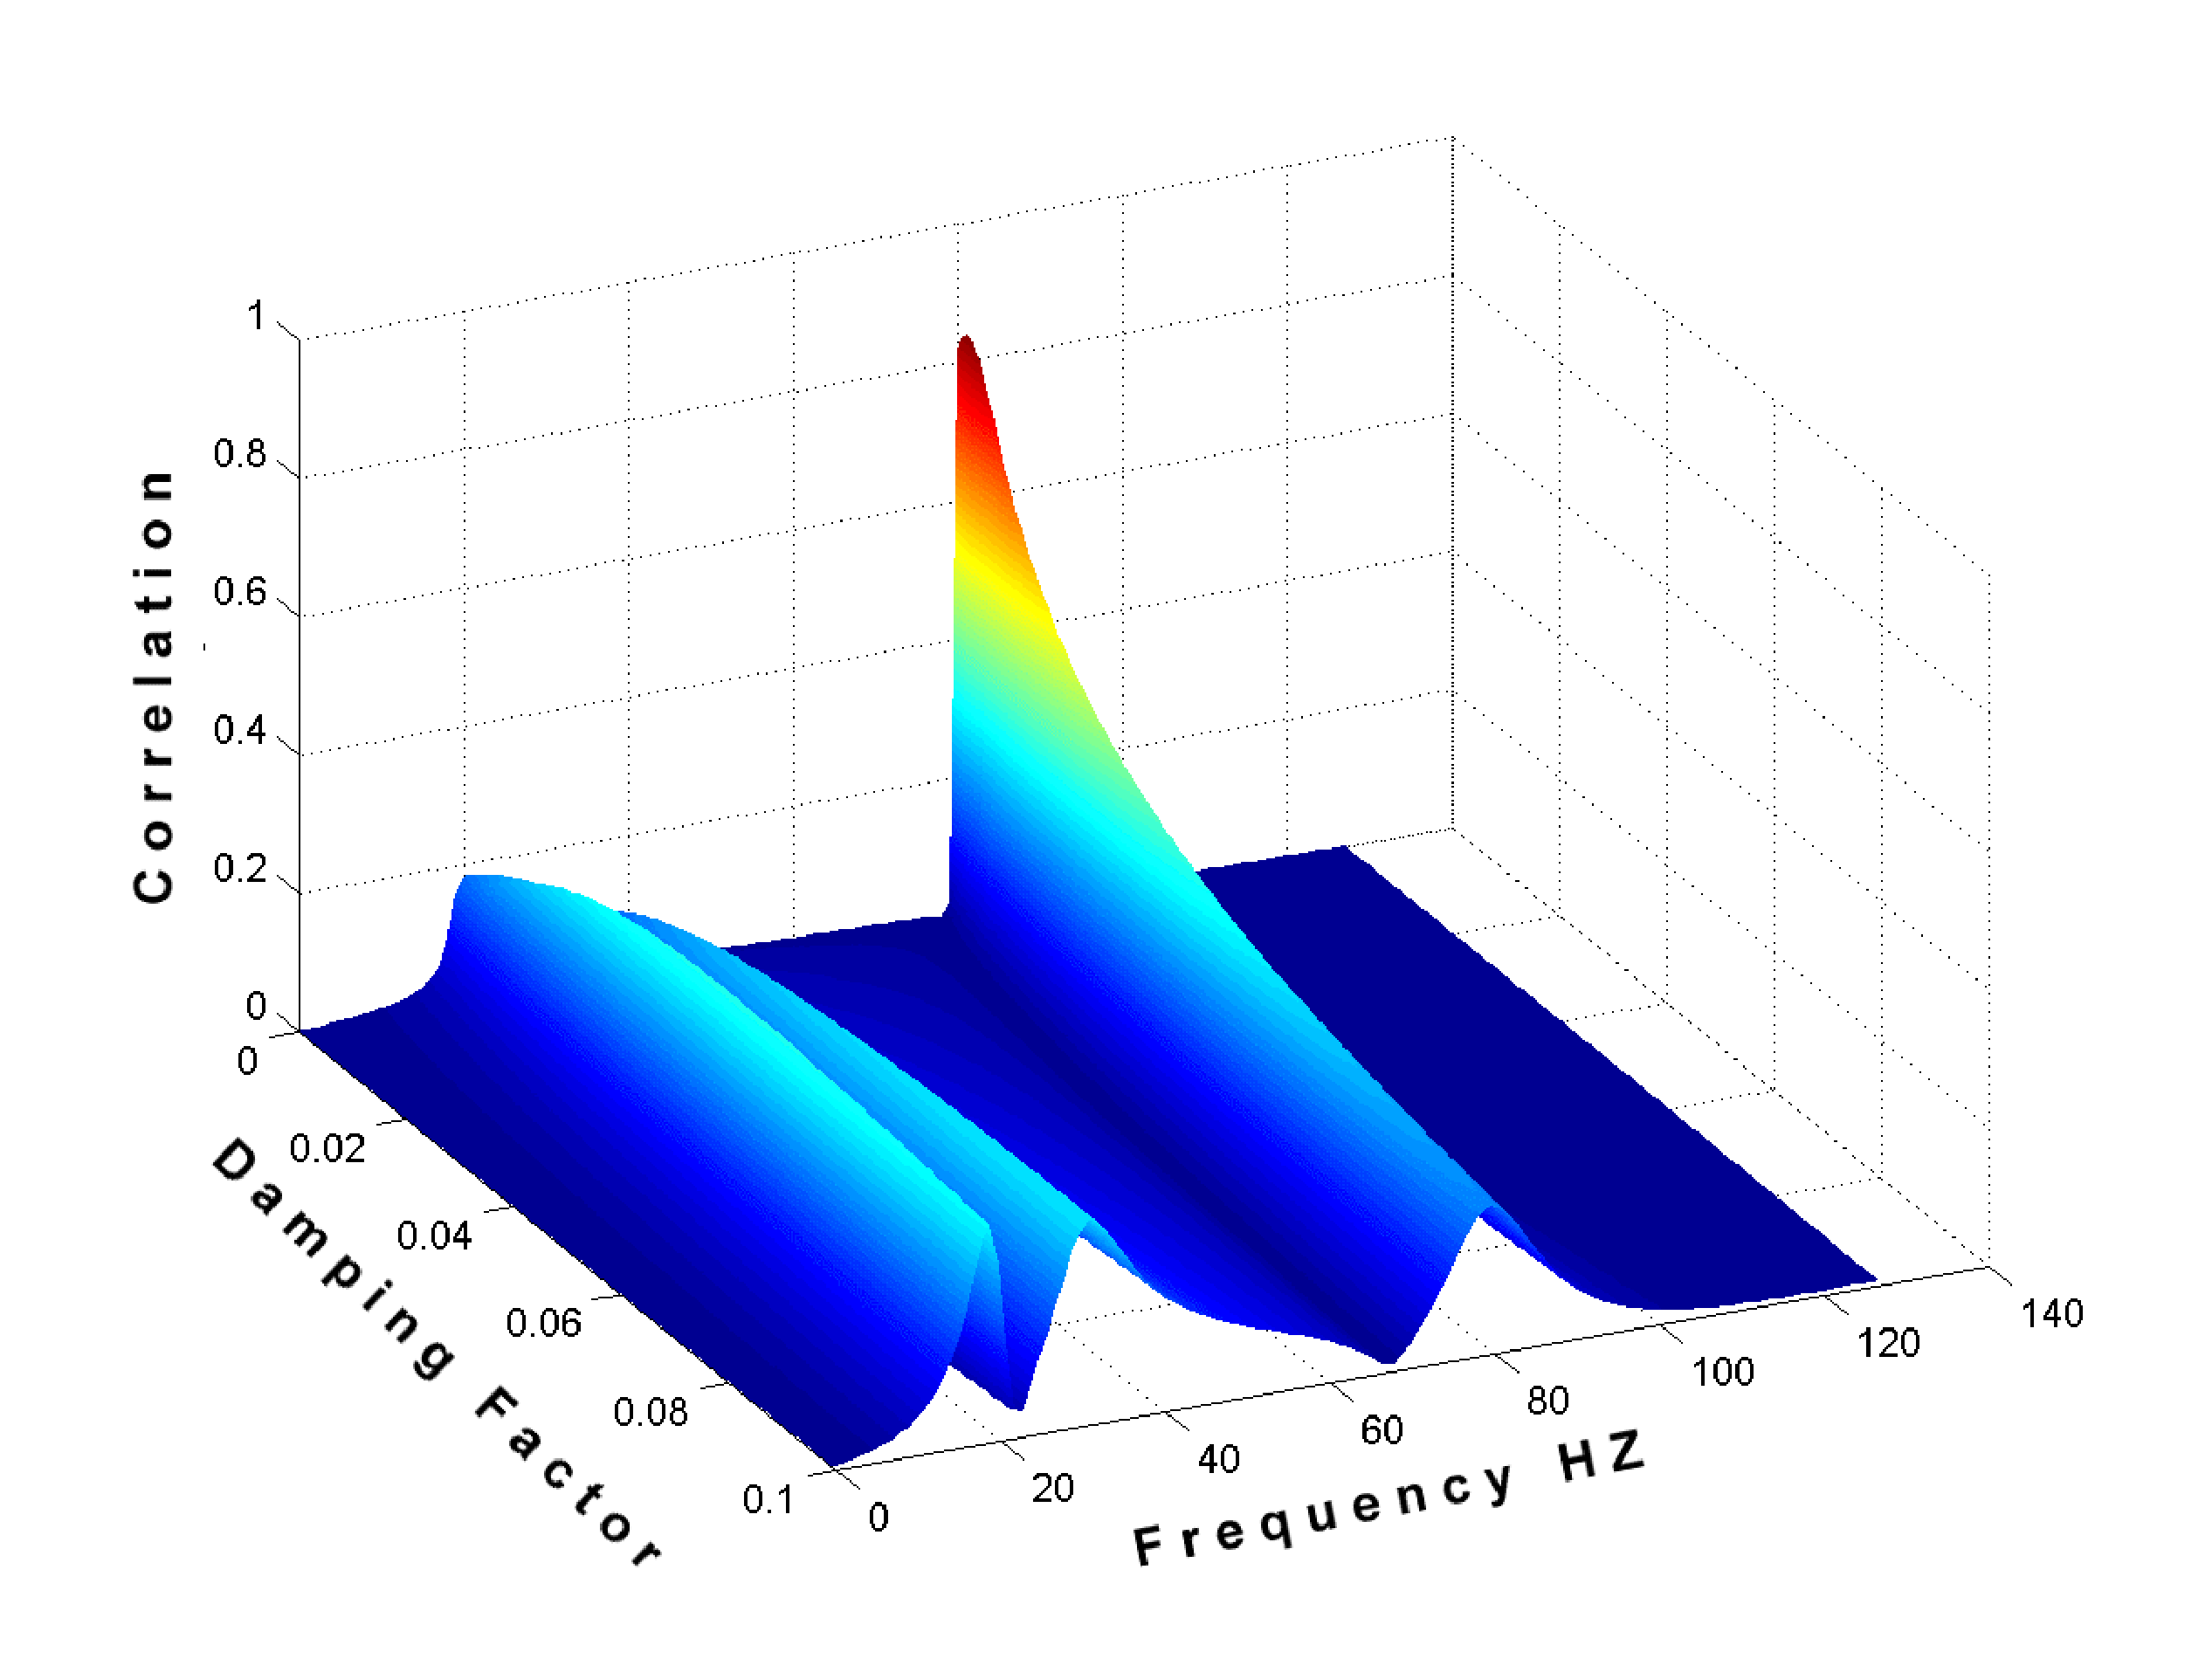
\includegraphics[keepaspectratio=true,scale=0.3]{figuras/fig01.eps}
	\caption{Wavelets correlation coefficients}
	\label{fig01}
\end{figure}

\section{Tabela}

As tabelas devem estar centradas entre margens e identificadas por uma legenda 
alinhada a esquerda, com recuo especial de deslocamento de 1,8 cm, posicionada 
acima da tabela com mostrado na Tab. \ref{tab01}, a título de 
exemplo. O tamanho das fontes empregadas nos rótulos e anotações usadas nas 
tabelas deve ser compatível com o usado no corpo do texto. Rótulos e anotações 
devem estar em português. Um espaçamento de 11 pts deve ser deixado entre a 
legenda e a tabela, bem como após a tabela. A numeração, a fonte e a formatação
são automáticas quando se usa o \LaTeX.

As grandezas dimensionais mostradas em cada tabela devem apresentar unidades 
consistentes com o SI. As unidades de cada variável devem ser mostradas apenas 
na primeira linha e/ou coluna da tabela, entre colchetes 

A referência explícita no texto à uma dada tabela deve ser feita como 
\lq\lq Tab. \ref{tab01}\rq\rq\ quando no meio de uma frase ou como 
\lq\lq Tabela \ref{tab01}\rq\rq\ quando no início da mesma. Referências 
implícitas a uma dada tabela devem ser feitas entre parênteses como 
(Tab. \ref{tab01}). Para referências a mais de uma tabela as mesmas 
regras devem ser aplicadas usando-se o plural adequadamente. Exemplos:
\begin{itemize}
	\item \lq\lq Após os ensaios experimentais, foram obtidos os resultados 
	mostrados na Tab. \ref{tab01}, que ...\rq\rq
	\item \lq\lq A Tabela \ref{tab01} apresenta os resultados obtidos, onde 
	pode-se observar que ...\rq\rq
	\item \lq\lq As Tabelas 1 a 3 apresentam os resultados obtidos, ...\rq\rq
	\item \lq\lq Verificou-se uma forte dependência entre as variáveis citadas 
	(Tab. \ref{tab01}), comprovando ...\rq\rq
\end{itemize}

Cada tabela deve ser posicionada o mais próxima possível da primeira citação 
feita à mesma no texto, imediatamente após o parágrafo no qual é feita a 
citação, se possível, na mesma página.

\begin{table}[h]
	\centering
	\caption{Propriedades obtidades após processamento}
	\label{tab01}
	
	\begin{tabular}{ccc}
		\toprule
		\textbf{Processing type} & \textbf{Property 1} (\%) & 
		\textbf{Property 2} $[\mu m]$ \\
		\midrule
		Process 1 & 40.0 & 22.7 \\
		Process 2 & 48.4 & 13.9 \\
		Process 3 & 39.0 & 22.5 \\
		Process 4 & 45.3 & 28.5 \\
		\bottomrule
	\end{tabular}
\end{table}

\section{Citação de Referências}

Referencias a outros trabalhos tais como artigos, teses, relatórios, etc. devem 
ser feitas no corpo do texto devem estar de acordo com a norma corrente ABNT 
NBR 6023:2002 (ABNT, 2000), esta última baseada nas normas ISO 690:1987:
\begin{itemize}
	\item \lq\lq \citeonline{bordalo1989}, mostraram que...\rq\rq

	\item \lq\lq Resultados disponíveis em \cite{coimbra1978}, \cite{clark1986} 
	e \cite{sparrow1980}, mostram que...\rq\rq
\end{itemize}

Para referências a trabalhos com até dois autores, deve-se citar o nome de 
ambos os autores, por exemplo: \lq\lq \citeonline{soviero1997}, mostraram 
que...\rq\rq

Para citação direta, o texto deve estar em fonte 10 com recuo de 4cm da margem esquerda:

\begin{citacao}
Foram desenvolvidos métodos eficazes de especificação, \textit{design} e implementação de software.  Novas notações e ferramentas reduziram o esforço necessário para produzir sistemas grandes e complexos \cite{Sommerville2007}.
\end{citacao}


% \chapter[Elementos do Pós-Texto]{Elementos do Pós-Texto}

Este capitulo apresenta instruções gerais sobre a elaboração e formatação dos 
elementos do pós-texto a serem apresentados em relatórios de Projeto de 
Graduação. São abordados aspectos relacionados a redação de referências 
bibliográficas, bibliografia, anexos e contra-capa.

\section{Referências Bibliográficas}

O primeiro elemento do pós-texto, inserido numa nova página, logo após o último 
capítulo do trabalho, consiste da lista das referencias bibliográficas citadas 
ao longo do texto.

Cada referência na lista deve ser justificada entre margens e redigida no 
formato Times New Roman com 11pts. Não é necessário introduzir uma linha em 
branco entre referências sucessivas.

A primeira linha de cada referencia deve ser alinhada a esquerda, com as demais 
linhas da referencia deslocadas de 0,5 cm a partir da margem esquerda. 

Todas as referências aparecendo na lista da seção \lq\lq Referências 
Bibliográficas\rq\rq\ devem estar citadas no texto. Da mesma forma o autor deve 
verificar que não há no corpo do texto citação a referências que por 
esquecimento não forma incluídas nesta seção.

As referências devem ser listadas em ordem alfabética, de acordo com o último 
nome do primeiro autor. Alguns exemplos de listagem de referencias são 
apresentados no Anexo I.

Artigos que ainda não tenham sido publicados, mesmo que tenham sido submetidos 
para publicação, não deverão ser citados. Artigos ainda não publicados mas que 
já tenham sido aceitos para publicação devem ser citados como \lq\lq in 
press\rq\rq.

A norma \cite{NBR6034:2000}, que regulamenta toda a formatação a ser usada na 
elaboração de referências a diferente tipos de fontes de consulta, deve ser 
rigidamente observada. Sugere-se a consulta do trabalho realizado por 
\cite{arruda2007}, disponível na internet.

\section{Anexos}

As informações citadas ao longo do texto como \lq\lq Anexos\rq\rq\ devem ser 
apresentadas numa seção isolada ao término do trabalho, após a seção de 
referências bibliográficas. Os anexos devem ser numerados seqüencialmente em 
algarismos romanos maiúsculos (I, II, III, ...). A primeira página dos anexos 
deve apresentar um índice conforme modelo apresentado no Anexo I, descrevendo 
cada anexo e a página inicial do mesmo.

A referência explícita no texto à um dado anexo deve ser feita como 
\lq\lq Anexo 1\rq\rq. Referências implícitas a um dado anexo devem ser feitas 
entre parênteses como (Anexo I). Para referências a mais de um anexo as mesmas 
regras devem ser aplicadas usando-se o plural adequadamente. Exemplos:
\begin{itemize}
	\item \lq\lq Os resultados detalhados dos ensaios experimentais são 
	apresentados no Anexo IV, onde ...\rq\rq

	\item \lq\lq O Anexo I apresenta os resultados obtidos, onde pode-se 
	observar que ...\rq\rq

	\item \lq\lq Os Anexos I a IV apresentam os resultados obtidos ...\rq\rq

	\item \lq\lq Verificou-se uma forte dependência entre as variáveis citadas 
	(Anexo V), comprovando ...\rq\rq
\end{itemize}



\bookmarksetup{startatroot} 

\postextual

\bibliography{bibliografia} 
\input{editaveis/11_apendices}
\input{editaveis/12_anexos}
% \begin{apendicesenv}

\partapendices

\chapter{Primeiro Apêndice}

Texto do primeiro apêndice.

\chapter{Segundo Apêndice}

Texto do segundo apêndice.

\end{apendicesenv}

% \begin{anexosenv}

\partanexos

\chapter{Primeiro Anexo}

Texto do primeiro anexo.

\chapter{Segundo Anexo}

Texto do segundo anexo.

\end{anexosenv}


\printindex

\end{document}

